\documentclass{classes/SIT-Report-EN}
\usepackage{tabularx}
\usepackage{amssymb}
\usepackage{colortbl}
\usepackage{graphicx}
\usepackage{adjustbox}
\usepackage{lscape}
\usepackage{longtable}
\usepackage{tabularray}
\usepackage{color}
\usepackage{multirow}
\usepackage{graphicx}
\usepackage[normalem]{ulem}
\usepackage{hyperref}
\usepackage{filecontents}

\useunder{\uline}{\ul}{}
 
%%Edit your info Here
\begin{document}
\title{PLANADAY : SUGGEST ONE DAY TRIP APPLICATION}
\degree{Bachelor of Science}
\majorProgramEN{Computer Science}
\academicyear{2024}

\author{Mr. Sitiporn Wimolpunyakul}
\authorTwo{MS. Kanyarant Premprapapong}
\authorThree{MS. Thanakorn Chotthanigarn}

\majoradvisor{Asst.Prof. Worarat Krathu}
% \coadvisor{Dr. Watanyoo Suksa-ngaim Ph.D}
\committeeOne{Dr. Watanyoo Suksa-ngiam}
\committeeTwo{Dr. Vithida Chongsuphajaisiddhi}
\academicyear{2024}

%%%%%%%%%%
\maketitle
\frontmatter
\maketitleinner
\makeapproval
% ************************** Thesis Abstract **********************************
\begin{abstract}
\par
PlanADay is a mobile application designed to generate personalized one-day trip plans
with minimal effort based on user preferences and input data. The application utilizes two
recommendation strategies: Most-Related Places From Location Area and Based-on-Preferences
Interests. Users can specify details such as their categories of interest (e.g., gyms, parks, cafes,
restaurants, museums, theaters, or art galleries), the starting date and time, preferred location
area, and the number of places to visit. Additionally, PlanADay allows users to view detailed
attraction information, bookmark plans, and access their plan history.
\par
\vspace{0.5cm}
This project demonstrates the practicality of implementing a plan suggestion system by
leveraging user inputs to tailor recommendations. The app provides an intuitive and engaging
experience, enabling users to efficiently discover and plan their ideal day while enhancing
satisfaction and utility.
\vfill
{Keywords :} Plan/ Interests / Mobile Application / Suggestion
\vfill
\end{abstract} %%Edit your Abstract
% ************************** Thesis Acknowledgements **************************
\begin{acknowledgements}
We received assistance and guidance from several respected persons, who deserve our deepest
gratitude. This project would not have been feasible without the support of Asst.Prof.Dr. Worarat
Krathu contributed invaluable insight and experience.
\par
\vspace{0.5cm}
In addition, we would also like to express our appreciation to Mr. Thanatat Wongabut and Ms.
Sukanya Chinwicha, and Mr. Ukrit Ruckcharti who generously contributed their time and
expertise to our project.
\end{acknowledgements} %% %%Edit your Acknowledgement

\tableofcontents
\listoftables
\listoffigures
%% ***************************** Thesis Symbols ********************************
\begin{symbols}
    \noindent
    \begin{tabular*}{\textwidth}{@{}p{0.18\textwidth}p{0.8\textwidth}@{}}
        {$\theta$} & {Theta} \\
        {$d$} & {distance} \\
        {kg} & {Kilogram} \\
        {m$^{2}$} & {Square Metre} \\
    \end{tabular*}
\end{symbols}
%% ************************** Thesis Abbreviations **************************
\begin{abbreviations}
    \noindent
    \begin{tabular*}{\textwidth}{@{}p{0.18\textwidth}p{0.8\textwidth}@{}}
        {DoF} & {Degree of Freedom} \\
        {CoM} & {Center of Mass} \\
        {KMUTT} & {King Mongkut's University of Technology Thonburi} \\
    \end{tabular*}
\end{abbreviations}


\mainmatter
%%insert your content
\chapter{Introduction}
\section{Background}
In today's fast-paced world, people rely more on technology to plan their daily activities and
their free time. However, many planning tools provide general suggestions that may not be
suitable for individual preferences or specific situational requirements such as time, location, or
interest activities. The growing demand for personalized planning in mobile applications gives
an opportunity to create a smart solution that personalizes recommendations to each user's
specific preferences. Users today expect convenience, accuracy, and relevance, especially when
it comes to planning their day or deciding where to go for activities. Personalized services are no
longer an option but rather a requirement for improving user satisfaction and engagement in an
increasingly digital era.
\section{Objectivs}
\begin{enumerate}
    \item To provide the plan which is suitable to the user’s preference.
    \item To provide up-to-date information on opening hours and availability.
\end{enumerate}

\section{Scope}
This project aims to develop a mobile application that suggests one-day trip plans based on user
interests, such as cafes, restaurants, shopping, parks, and more. Users can also provide input,
such as starting location, date and time, and the number of places to visit, to refine the
suggestions and include more relevant locations in their plans. Users of the PlanADay
application
\begin{itemize}
    \item \textbf{can create} personalized one-day trip itineraries based on their interests and preferences.
    \item \textbf{can discover} nearby attractions that align with their preferences and current location.
    \item \textbf{can adjust} their generated plans by rearranging locations, deleting stops, or regenerating.
    \item \textbf{can view} detailed information for each suggested location.
    \item \textbf{can share} their trip plans with others on the platform.
    \item \textbf{can bookmark} plans created by other users for easy access and reference in the future.
    \item \textbf{can explore} their plan history to revisit past itineraries or gain inspiration for new trips.
\end{itemize}
\newpage

\section{Expected Benefits}
\begin{enumerate}
    \item \textbf{Seamless Trip Planning:} The main features of the application will help users to create
    their personal preferences, ensuring a tailored and enjoyable experience.
    \item \textbf{User Satisfaction and Flexibility:} Users will appreciate both the thoughtfully generated
    plans and the ease of customizing them to suit their needs, ensuring a more satisfying
    experience.
    \item \textbf{Business Partnerships:} By featuring related points of interest, such as shops and cafes,
    PlanADay opens opportunities for businesses to partner and connect with a highly
    engaged audience.
\end{enumerate}

\chapter{Feasibility}
\section{Introduction}

\par
Our transportation application aims to enhance user experience by providing seamless navigation from the starting point to the destination. In addition to providing efficient routes, we also offer transparent pricing information, allowing users to select the transportation method that best suits their budget. Our navigator displays the actual cost of each route, enabling users to make informed decisions and pay only for the transportation they use. In addition, we provide the mini social media in the application, users can also share their recent transportation methods to the mini community so that other users can view them.
\section{Problem Statement}
\begin{figure}[!h]
    \centering
    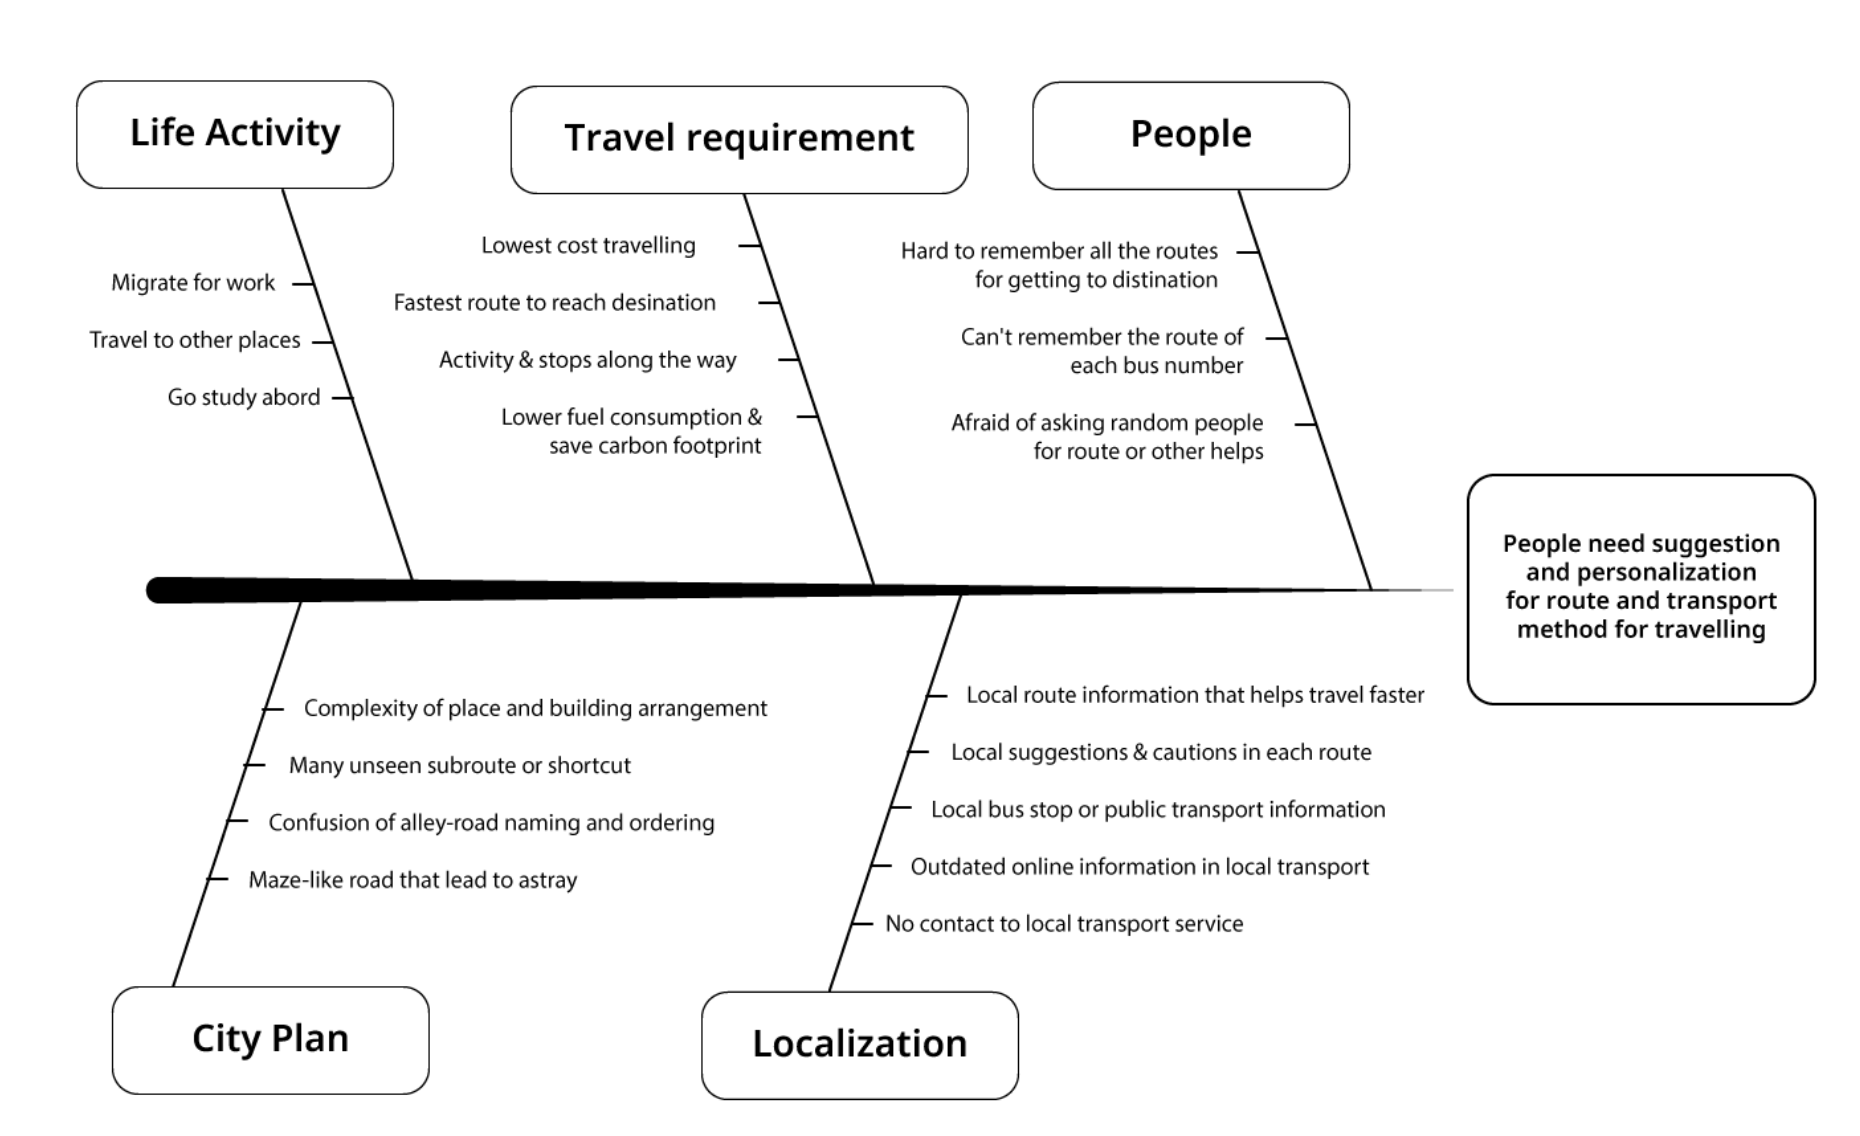
\includegraphics[width=0.8\linewidth]{chapter2/problem-statement.png}
    \caption{Problem diagram}    
    \label{fig:Problem diagram}
\end{figure}
\par
In people's everyday life, they need to transport to places for doing things, from daily commute to work, go on a trip or even going abroad. However, there's many concerning and obstacle for transportation. People themselves not able to remember all the routes (i.e., transportation line) that bring him to destination or sometimes there might be more better (in terms of cost, duration, or transfer) transportation route for them that they don't know. These problem may influenced by city plan that have complex arrangements or some localization that might leads to misinformation. As transportation, especially public transportation has a important impact to  people, improving transport information to be more accurate, accessible, and personalized will give an opportunity to people for more ease of life, so all these reasons lead to why we need a better routing application.

\newpage
\section{Related Research Projects}
\subsection{Google Maps}
This application is designed for regular users who use to find the location of the place, and transportation method between one point to another point, Google Maps allows users to see the detail of the traffic and estimate the time of transporting in each way that user select.
\begin{figure}[!h]
    \centering
    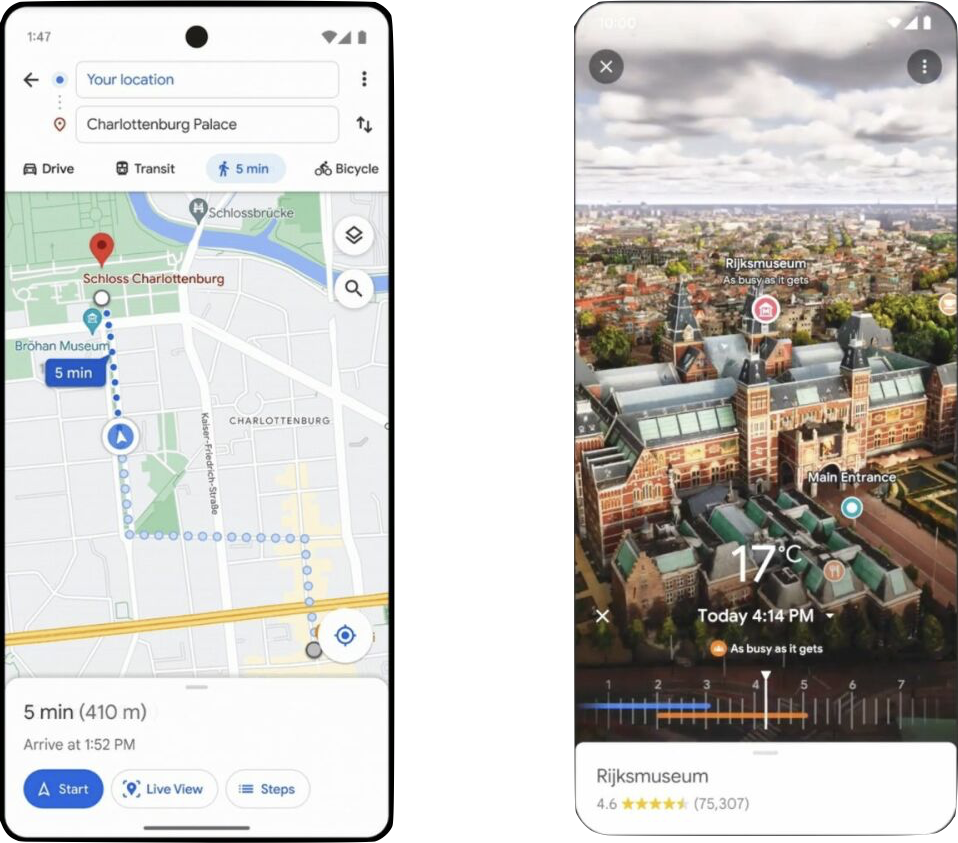
\includegraphics[width=0.5\linewidth]{chapter2/google_map.png}
    \caption{The Google Maps application}
    \label{fig:The Google Maps application}
\end{figure}

\subsection{Apple Maps}
This application is for Apple users that allows users to find the location, the way to go to their destination, estimate the time of transportation, see the details of traffic, and Apple Maps also provides the bicycle method, so cyclists can use Apple Maps to find the best way to get to their destination by bicycle.
\begin{figure}[!h]
    \centering
    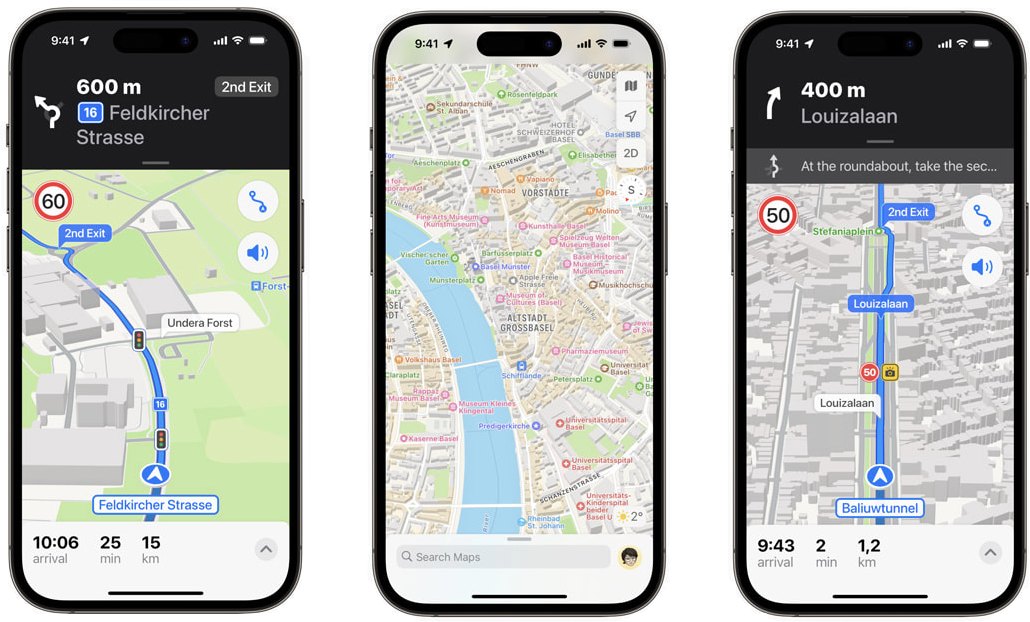
\includegraphics[width=0.5\linewidth]{chapter2/apple_map.png}
    \caption{The Apple Maps application}
    \label{fig:The Apple Maps application}
\end{figure}

\newpage
\subsection{ViaBus}
\par
ViaBus application is the application that provides user with the bus stops and routes, real-time bus locations approaching your stop, and recommended routes to travel from one place to another place which include buses, trains, and boats.
\begin{figure}[!h]
    \centering
    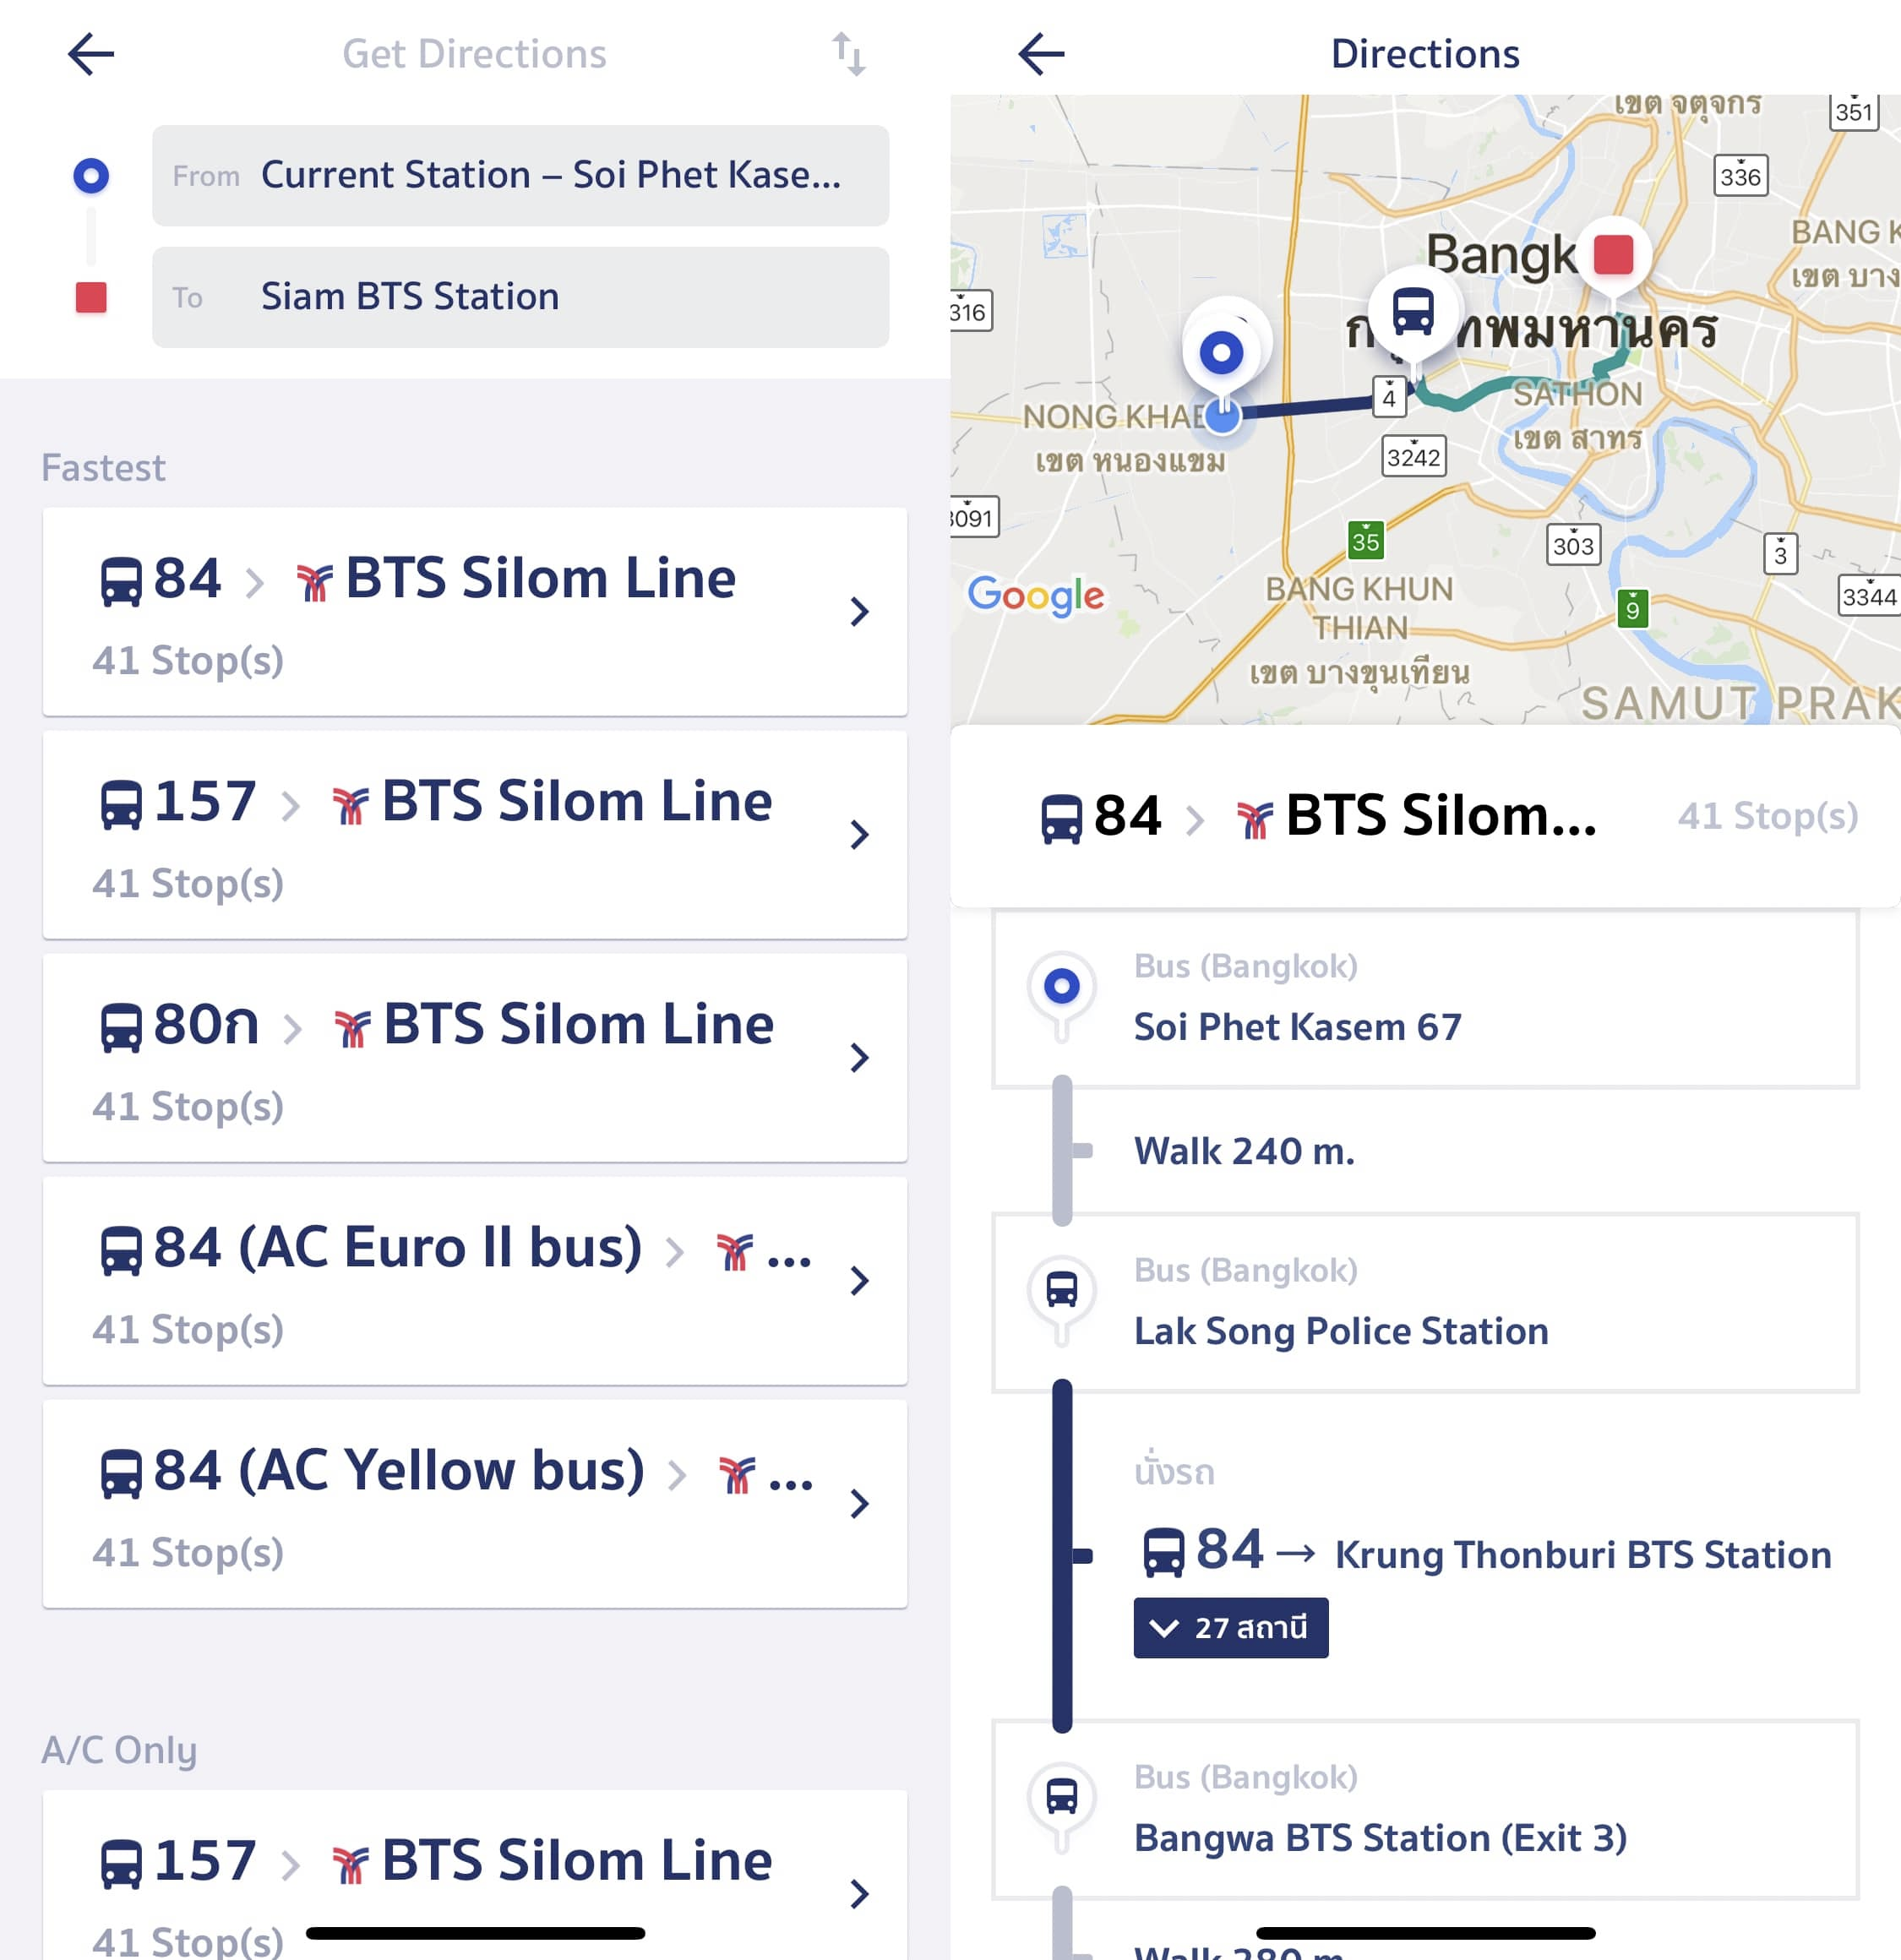
\includegraphics[width=0.5\linewidth]{chapter2/viabus.png}
    \caption{The ViaBus application}
    \label{fig:The ViaBus application}
\end{figure}

%---------------------------------------------------------------%
\subsection{Existing Functions}
\begin{table}[!h]
	\centering
	\resizebox{\linewidth}{!}{%
		\begin{tabular}{|>{\centering\hspace{0pt}}m{0.104\linewidth}|>{\centering\hspace{0pt}}m{0.085\linewidth}|>{\centering\hspace{0pt}}m{0.154\linewidth}|>{\centering\hspace{0pt}}m{0.173\linewidth}|>{\centering\hspace{0pt}}m{0.144\linewidth}|>{\centering\hspace{0pt}}m{0.142\linewidth}|>{\centering\arraybackslash\hspace{0pt}}m{0.129\linewidth}|} 
			\hline
			Applications & Map route & Search for destination & Routes recommendation & Estimate travel time & Estimate travel cost & Record travel info  \\ 
			\hline
			Google Maps  & Yes       & Yes                    & Yes                   & Yes                  & No                   & Yes                 \\ 
			\hline
			Apple Maps   & Yes       & Yes                    & Yes                   & Yes                  & No                   & Yes                 \\ 
			\hline
			ViaBus       & Yes       & Yes                    & No                    & No                   & No                   & No                  \\ 
			\hline
			TravelKit    & Yes       & Yes                    & Yes                   & Yes                  & Yes                  & Yes                 \\
			\hline
		\end{tabular}
	}
	\caption{Existing functions of related research application and TravelKit}
\end{table}

\newpage
\section{Requirement Specifications}
\subsection{System requirements}
\begin{itemize}
	\item Users select the destination after that the map view shows the path to travel to the destination, the estimated cost of traveling, and the estimated time to get there and the user can select the best way for them.
	\item Record the selected path from the user.
	\item Create the graph that provides the way to travel to the destination.
	\item Estimate the time from the one place to another place based on the path that is selected by the user.
	\item Estimate the cost on the selected path.
	\item Users can start and stop their trip.
	\item After a trip has been recorded, the application will record it in the database.
\end{itemize}

\subsection{Mobile application requirements}
\begin{itemize}
	\item Smartphone with Android OS or iOS
	\item Has geo-positioning sensor (GPS)
\end{itemize}

\section{Implementation Technique}
\begin{itemize}
	\item Frontend
	\begin{itemize}
		\item Programming language: Dart
		\item UI SDK: Flutter
		\item HTTP Client: Dio
	\end{itemize}
	\item Backend
		\begin{itemize}
		\item Go Runtime
		\item GoFiber for API server
	\end{itemize}
	\item Database Server
	\begin{itemize}
		\item MySQL: Persistent and relational data store
		\item MongoDB: Document Database for storing transport data
		\item Neo4j: Graph database for routing and path finding
	\end{itemize}
	\newpage
	\item 3rd party API
	\begin{itemize}
		\item Firebase Authentication: Sign-in and credential management
		\item Google Maps API: Geographic information retrieval
		\item OSRM: Routing engine for shortest paths in road networks
	\end{itemize}
	\item Infrastructure
	\begin{itemize}
		\item Container management: Docker
		\item DNS: Cloudflare
	\end{itemize}
	\item Development Software
	\begin{itemize}
		\item Visual Studio Code
		\item Goland
		\item DataGrip
		\item Postman
		\item iOS, Android simulator
	\end{itemize}
	\item Others
	\begin{itemize}
		\item Version Control: GitLab
		\item User interface design: Figma
	\end{itemize}
\end{itemize}

\section{Deliverables}
\subsection{Application}
\begin{itemize}
	\item Source code of application
	\item Mobile application
\end{itemize}
\subsection{Documentation}
	\begin{itemize}
	\item Project report
	\item Meeting log
	\item Poster
\end{itemize}

\newpage
\section{Implementation Plan}
\begin{figure}[!h]
	\centering
	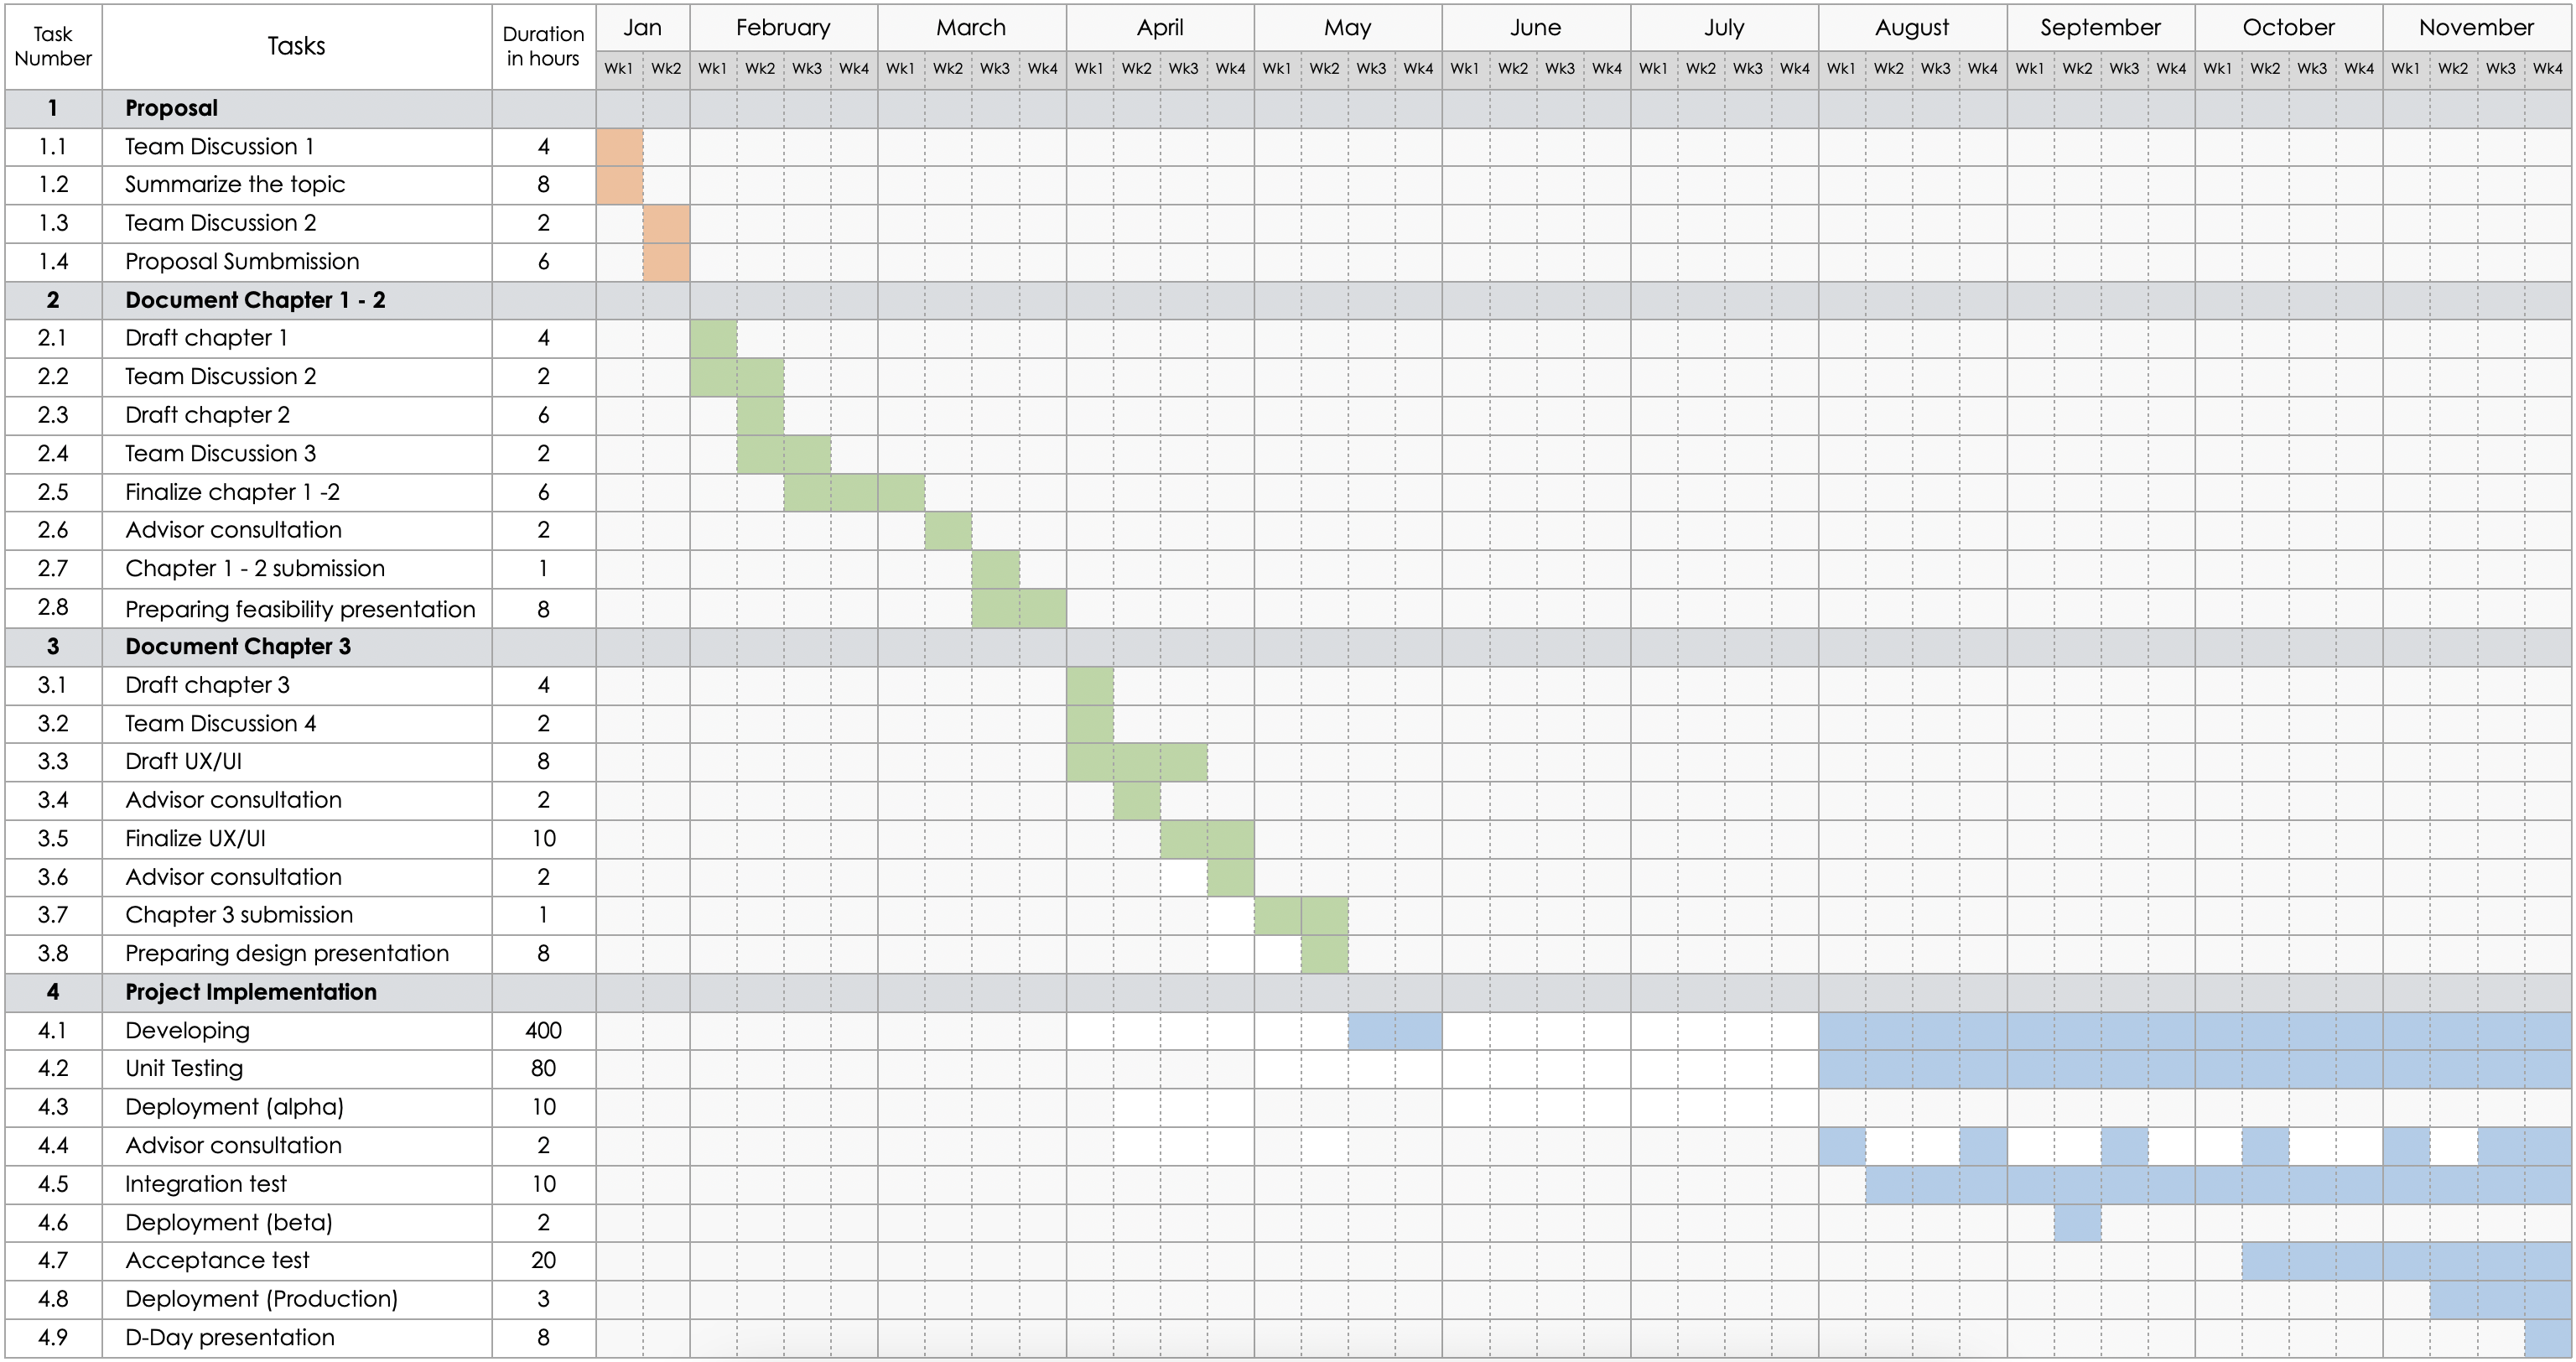
\includegraphics[width=1\linewidth]{chapter2/gantt_chart.png}
	\caption{Gantt Chart of the implementation plan}
	\label{fig:Gantt Chart of the implementation plan}
\end{figure}
\par
Our Implementation plan is divided into 4 phases that includes:
\begin{itemize}
	\item \textbf{Proposal Phase} During this initial stage, we engage in discussions to determine and finalize the topic for our project.
	\item \textbf{Document Chapter 1-2} In this phase, we delve into the conceptualization of ideas, feasibilities, conduct research, identify target users, and consult with advisors to gather essential information.
	\item \textbf{Document Chapter 3} This phase is dedicated to the creation of the project document, encompassing the development of diagrams, user personas, and the design of our application's user interface.
	\item \textbf{Project Implementation} The final phase involves a concentrated effort on coding, testing, and deploying our application.
\end{itemize}
\chapter{Analysis and Design}
\section{Introduction}
\par
This chapter provides an explanation of our project design in the following sections: analysis of
the existing system, user requirement analysis, and system design. First is analysis of the existing
system, this section evaluates the current systems and applications available in the market,
identifying their features, limitations, and areas for improvement along with the PlanADay
application. Second,the user requirement analysis section that explains the features of the project.
Third, the system design user diagrams consist of a context diagram, data flow diagram, activity
diagram, use case diagram, system sequence diagram, flow chart, and key-valued database
diagram.

\section{Analysis of the existing system}
Currently, several applications are available in the market that assist users in planning trips, such
as Google Maps, Strippl, Gethergo, and ChatGPT. These platforms offer various features,
including route navigation, attraction suggestions, and itinerary planning. However, they differ in
their ability to cater to specific user needs.
\par
For instance, most existing applications, like Google Maps and Strippl, are well-suited for users
who already know where they want to go, as they provide efficient routing paths and
location-based directions. Similarly, Gethergo offers recommendations based on user-defined
interests but requires users to input detailed preferences or destinations. On the other hand,
PlanADay offers catering to users who may not have a clear idea of where they want to go. The
application generates personalized, one-day trip plans based on broad user interests, preferences,
and current location, offering a complete itinerary without requiring extensive input or prior
knowledge of specific destinations. The comparison table below summarizes the key features of
each application.

\newpage
\begin{table}[]
    \begin{tabular}{|l|c|c|c|c|c|}
    \hline
    \rowcolor[HTML]{C0C0C0} 
    Feature                                                                                       & \multicolumn{1}{l|}{\cellcolor[HTML]{C0C0C0}Strippl} & \multicolumn{1}{l|}{\cellcolor[HTML]{C0C0C0}gethergo} & \multicolumn{1}{l|}{\cellcolor[HTML]{C0C0C0}Google Map} & \multicolumn{1}{l|}{\cellcolor[HTML]{C0C0C0}ChatGPT} & \multicolumn{1}{l|}{\cellcolor[HTML]{C0C0C0}PlanADay} \\ \hline
    Require less input                                                                            & \checkmark                                           & -                                                     & \checkmark                                              & -                                                    & \checkmark                                            \\ \hline
    \begin{tabular}[c]{@{}l@{}}Suggest plan base on user\\ interests and preferences\end{tabular} & -                                                    & \checkmark                                            & -                                                       & \checkmark                                           & \checkmark                                            \\ \hline
    Suggest route based on location                                                               & \checkmark                                           & \checkmark                                            & \checkmark                                              & -                                                    & \checkmark                                            \\ \hline
    Real-time place Details                                                                       & -                                                    & \checkmark                                            & \checkmark                                              & -                                                    & \checkmark                                            \\ \hline
    Provide routing path                                                                          & \checkmark                                           & \checkmark                                            & \checkmark                                              & -                                                    & \checkmark                                            \\ \hline
    Generate/ Regenerate plan                                                                     & -                                                    & -                                                     & -                                                       & \checkmark                                           & \checkmark                                            \\ \hline
    Save related plan from others                                                                 & \checkmark                                           & \checkmark                                            & \checkmark                                              &                                                      & \checkmark                                            \\ \hline
    Overview Detail                                                                               & -                                                    & \checkmark                                            & \checkmark                                              & -                                                    & \checkmark                                            \\ \hline
    \end{tabular}
    \caption{Table of the feature comparisons}
    \label{tab:my-table}
\end{table}
\par
The PlanADay application aims to address these limitations by offering a more personalized and
flexible experience. It not only generates customized one-day trip plans based on user interests
but also allows users to adjust itineraries, share plans with others in the community, and
bookmark suggestions for future use. By bridging these gaps, PlanADay seeks to provide a more
user-focused and collaborative solution compared to existing systems.

\section{User requirement analysis}
The user requirement analysis aims to identify the expectations, preferences, and functional
needs of users who seek efficient and personalized one-day trip planning. Below is a breakdown
of the key user requirements that they might found:
\begin{enumerate}
    \item Users do not get the satisfied plan from the user’s input.
    \begin{itemize}
        \item Customization plan: Users can edit the plan which is delete the place, add more
        places, and reorder the place on their own again to make the most appropriate
        plan for the user.
    \end{itemize}
    \item Users want to change their preferences.
    \begin{itemize}
        \item Preference setting: Users can reselect their preferences all the time in application.
    \end{itemize}
    \item Users do not have any specific input.
    \begin{itemize}
        \item Suggestion plan: The application provides the plan that are generated from other
        users, so the user can use other’s plan to travel.
    \end{itemize}
\end{enumerate}
\newpage
\section{System Design}
\subsection{Use case diagram}
\begin{figure}[!h]
    \centering
    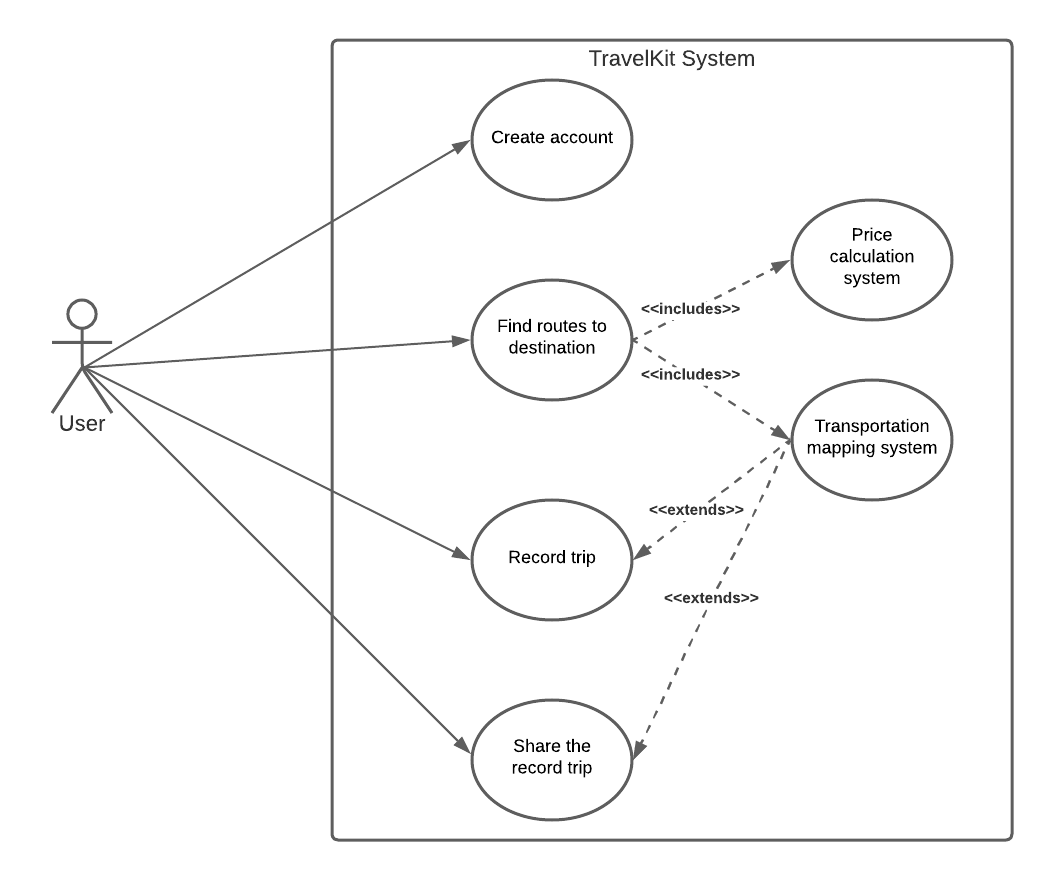
\includegraphics[width=0.7\linewidth]{chapter3/use-case-diagram.png}
    \caption{Use case diagram}
    \label{fig:Use case diagram}
\end{figure}
\par
The Actors who are in the PlanAday System. The user must create the account to authenticate in
the system. After the user input all field forms to create a plan, including the plan name, place
type, location, date and time and amount of places, The system will generate the plan and
display it to the user. if the user is not satisfied they can customize the plan by rearrange,
regenerate. The suggestion plans will show the public plans that mean each plan is shared by
other users. and filter the plan by user preferences.
\newpage
\subsection{Context diagram}
\begin{figure}[!h]
    \centering
    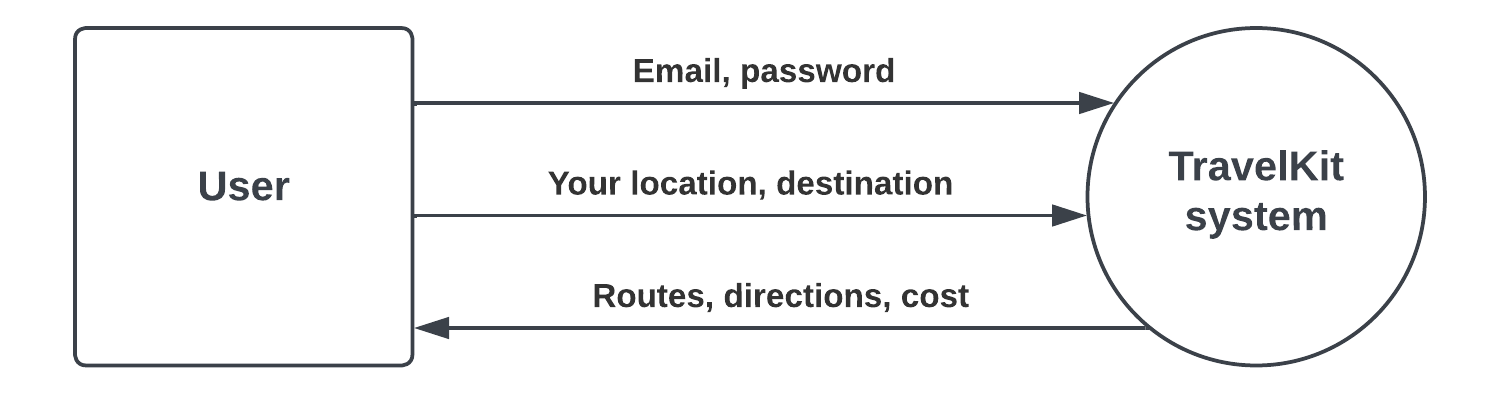
\includegraphics[width=1\linewidth]{chapter3/context-diagram.png}
    \caption{Context diagram}
    \label{fig:Context diagram}
\end{figure}
\par
The context diagram shows the overall of PlanADay System that requires the username,
password that need to be used in authentication service, place categories, location, date and time,
amount of places that need to be used in generating the plan. Then the system will provide a plan
that matches with input that includes details.

\newpage
\subsection{Activity Diagram}
Authentication process
\begin{figure}[!h]
    \centering
    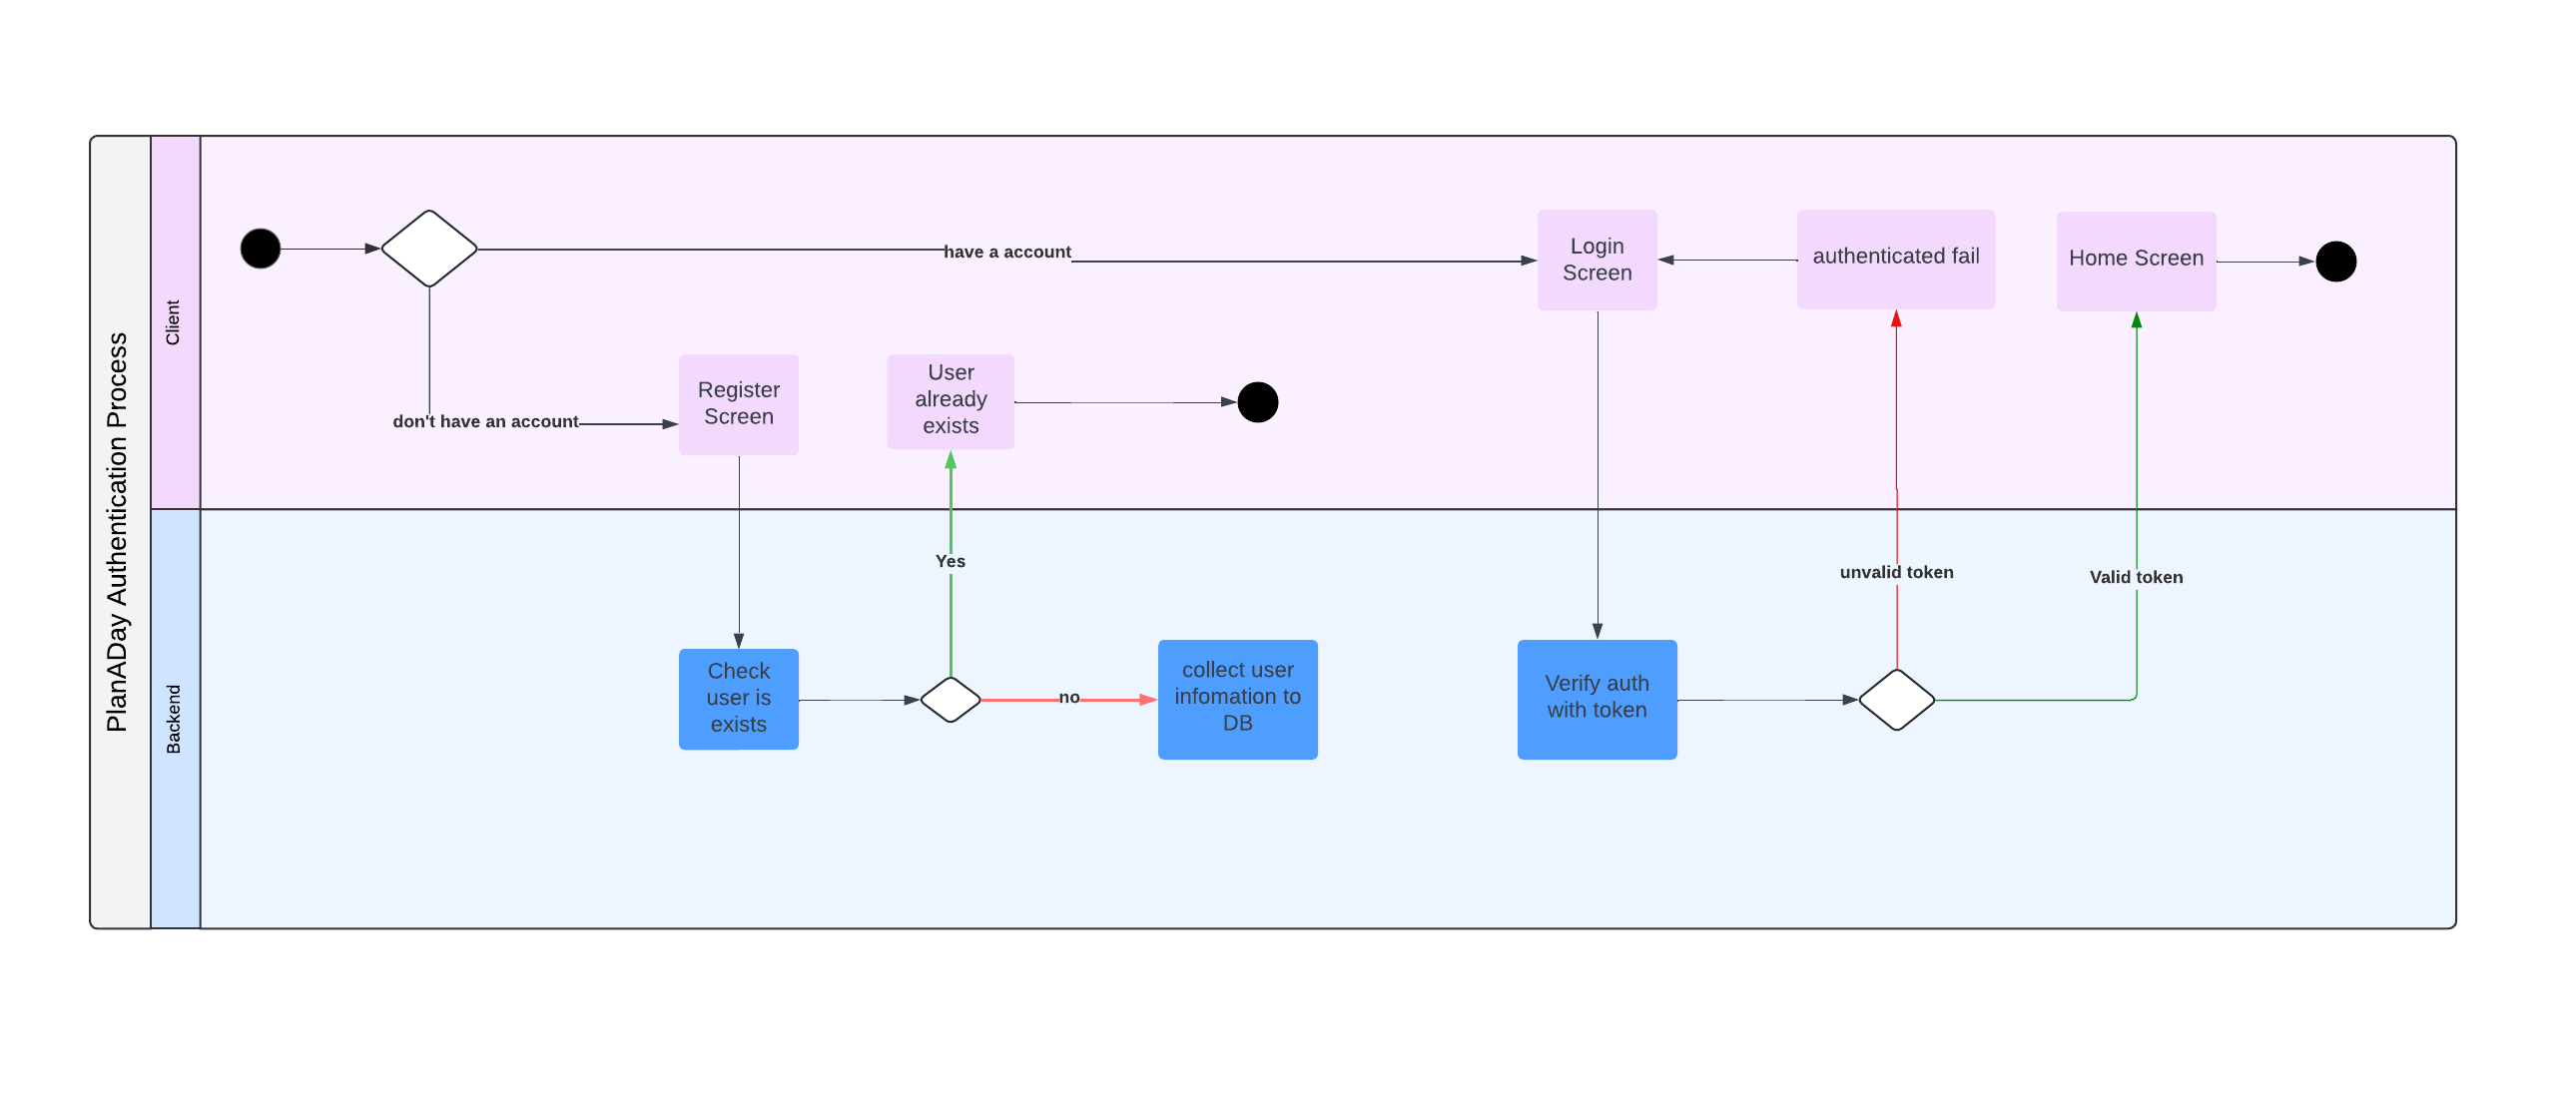
\includegraphics[width=1\linewidth]{chapter3/authentication-process.png}
    \caption{Activity Diagram of Authentication Process}
    \label{fig:Activity Diagram of Authentication Process}
\end{figure}
\par
The PlanADay Authentication Process illustrates the workflow for user registration and login,
divided into client-side and backend interactions. The process begins with a decision: if the user
does not have an account, they are directed to the registration screen. On registering, the backend
checks if the user already exists. If the user exists, they are informed and redirected to the login
screen; otherwise, their information is collected and stored in the database. For users with an
account, the login screen allows them to authenticate. The backend verifies the authentication
using a token. If the token is valid, the user is granted access to the home screen. In the event of
an invalid token, authentication fails. This flow ensures a secure and user-friendly mechanism
for handling account creation and login.
\newpage
Generate Plan Process
\begin{figure}[!h]
    \centering
    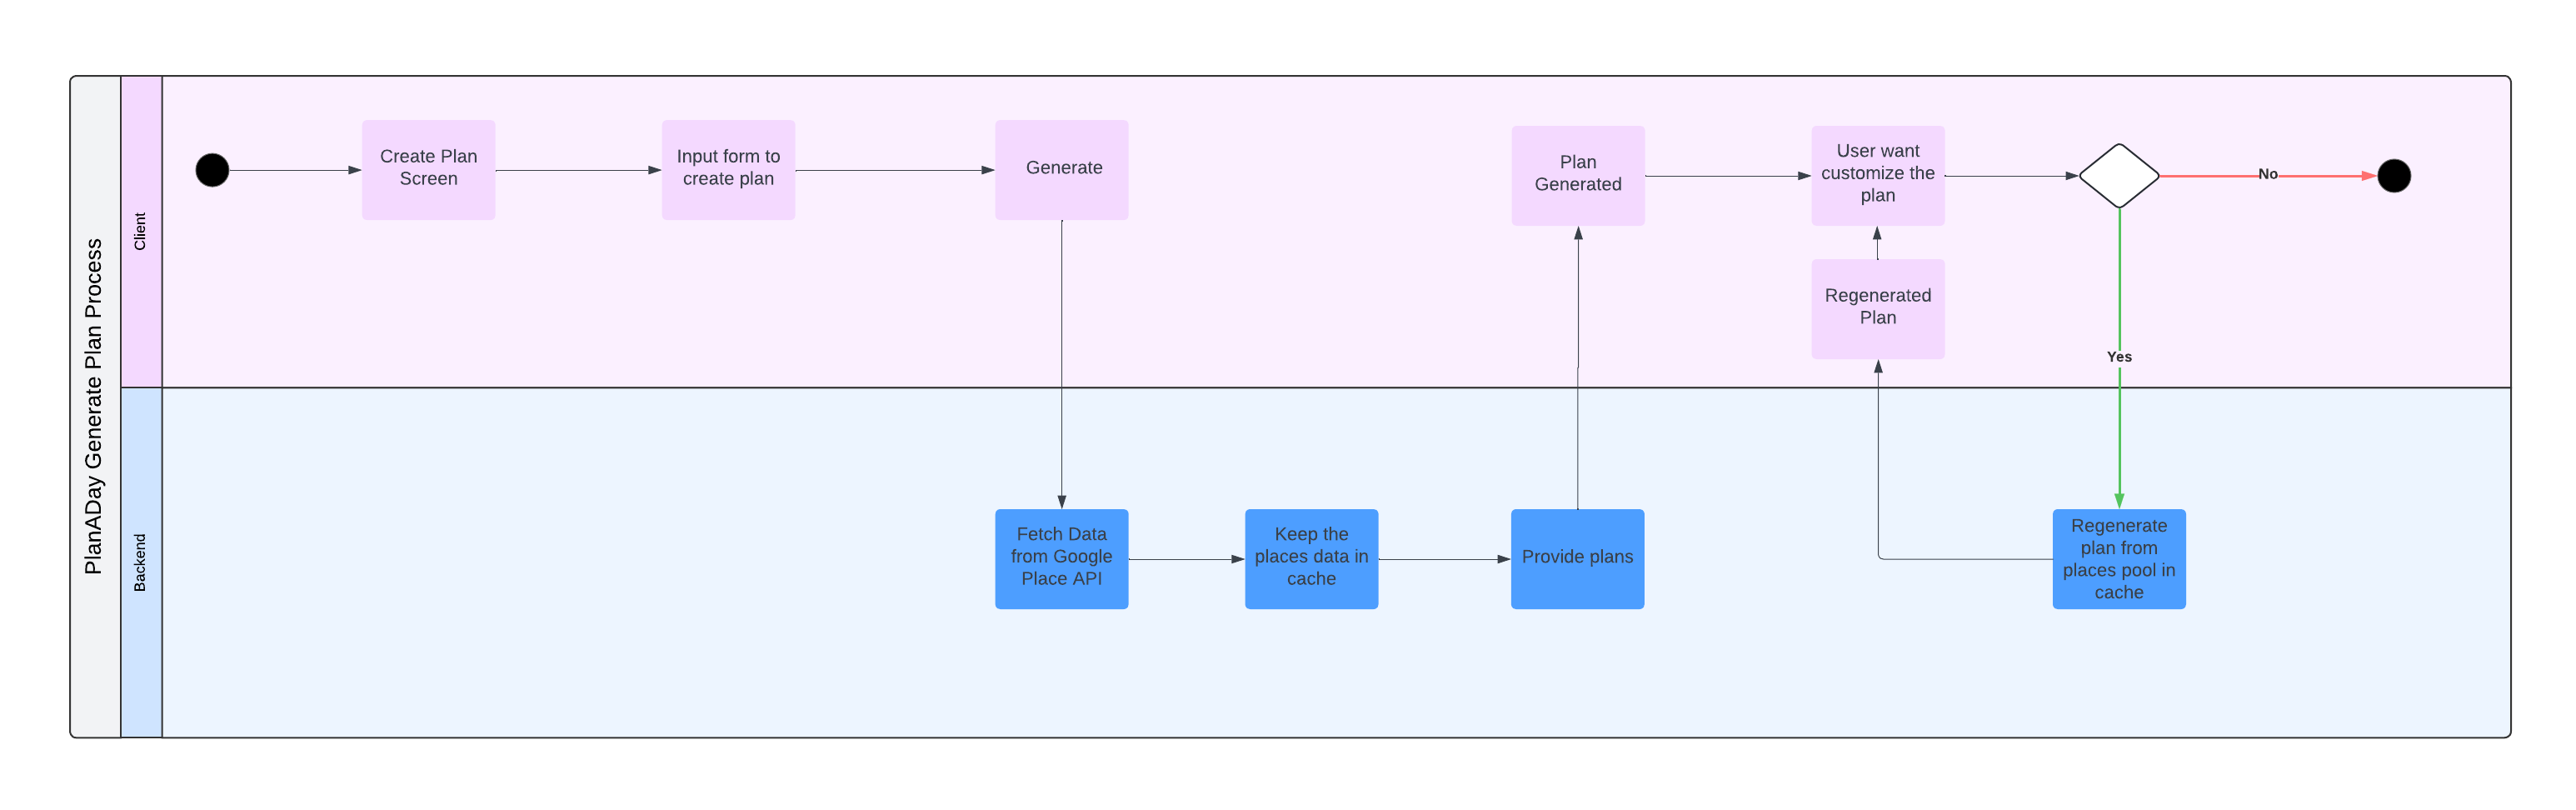
\includegraphics[width=1\linewidth]{chapter3/generate-process.png}
    \caption{Activity Diagram of Generate Plan Process}
    \label{fig:Activity Diagram of Generate Plan Process}
\end{figure}
\par
The PlanADay Generate Plan Process outlines the workflow for creating and customizing
plans. The process begins on the client side, where the user accesses the "Create Plan" screen,
fills out an input form, and initiates the plan generation. The backend fetches relevant data from
the Google Places API, caches the data for future use, and provides the generated plan to the
client. After the plan is displayed, the user has the option to customize it. If they choose to do so,
the backend regenerates the plan using the cached data without making additional API calls. If
no customization is needed, the process ends. This workflow ensures efficiency through caching
and provides a seamless user experience for generating personalized plans.
\newpage
\subsection{User Interface Design}

\begin{figure}[!h]
    \centering
    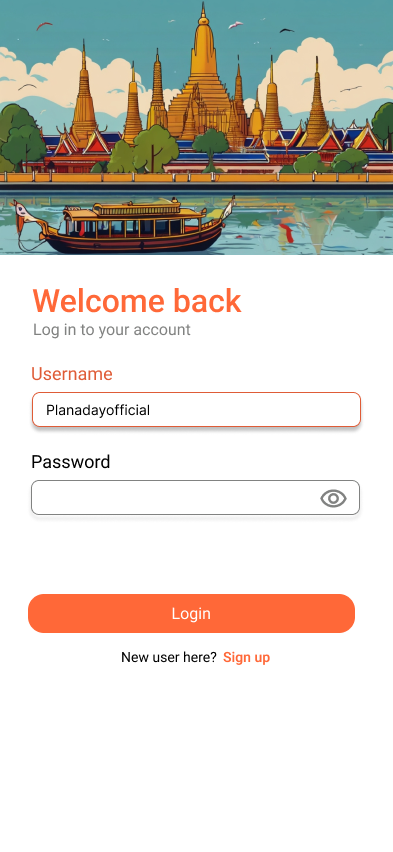
\includegraphics[width=0.5\linewidth]{chapter3/UI_Login_page.png}
    \caption{Login Page}
    \label{fig:Login Page}
\end{figure}
\noindent
Figure 3-5. display the Login page of PlanADay application. The system requires
the user to login using username and password for authentication.

\newpage
\begin{figure}[!h]
    \centering
    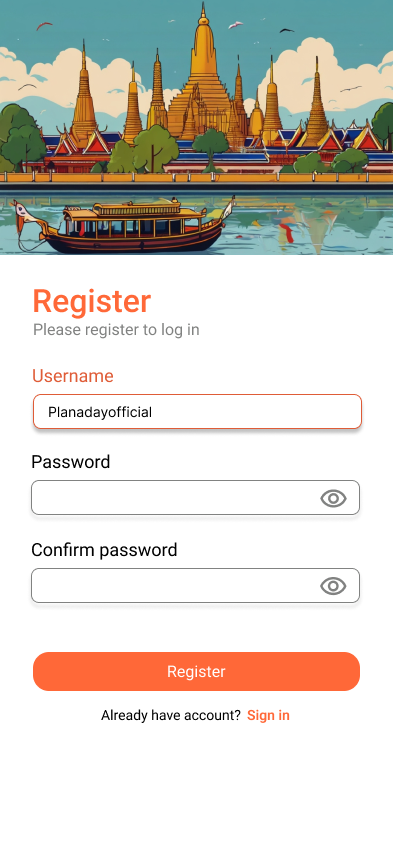
\includegraphics[width=0.5\linewidth]{chapter3/UI_Register_page.png}
    \caption{Register Page}
    \label{fig:Register Page}
\end{figure}
\noindent
Figure 3-6. display the Register page of PlanADay application. When users get in
the application for the first time, they are required to create the account to use in the
system.

\newpage
\begin{figure}[!h]
    \centering
    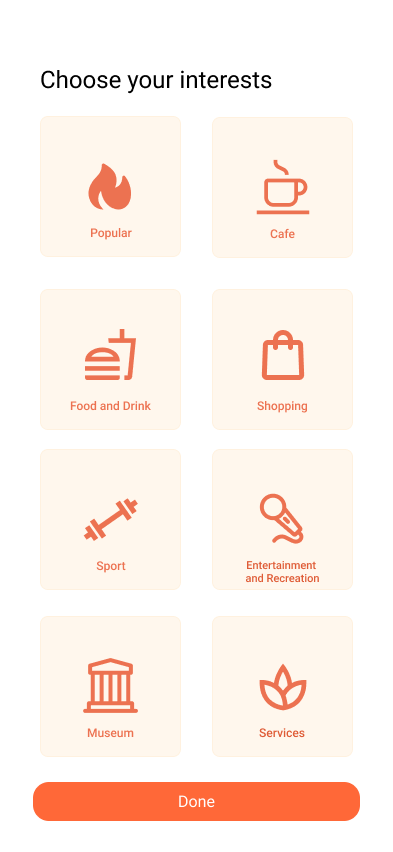
\includegraphics[width=0.5\linewidth]{chapter3/UI_Persona_page.png}
    \caption{Persona Page}
    \label{fig:Persona Page}
\end{figure}
\noindent
Figure 3-7. display the Persona page of PlanADay application. Users can set their
preferences in this page and it will be used to suggest the plan in the system.

\newpage
\begin{figure}[!h]
    \centering
    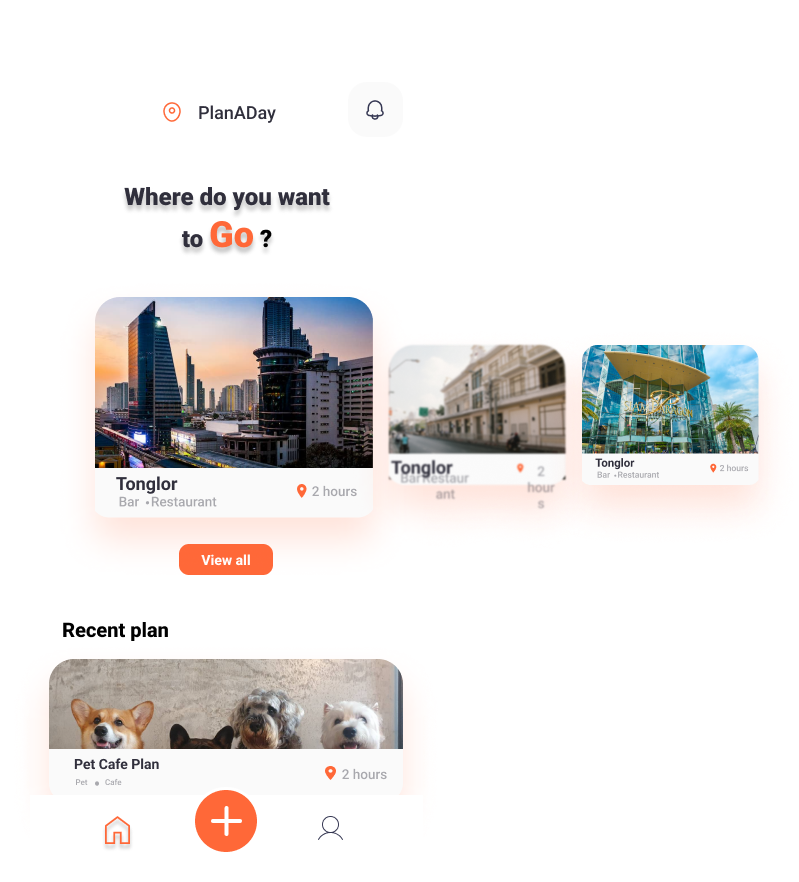
\includegraphics[width=1\linewidth]{chapter3/UI_Home_page.png}
    \caption{Home Page}
    \label{fig:Home Page}
\end{figure}
\noindent
Figure 3-8. display the Homepage of PlanADay application. The application will
show the plan suggestion and the plan that the user created in this page.

\newpage
\begin{figure}[!h]
    \centering
    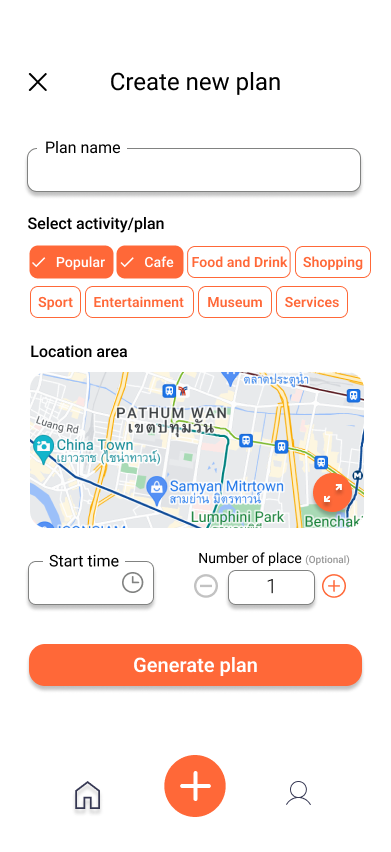
\includegraphics[width=0.5\linewidth]{chapter3/UI_Create_plan.png}
    \caption{Home Page}
    \label{fig:Home Page}
\end{figure}
\noindent
Figure 3-9. display the Create Plan page of PlanADay application. Users can create
their own plan on this page. The input are plan name, categories, location area, start
date, start time, and number of places.

\newpage
\begin{figure}[!h]
    \centering
    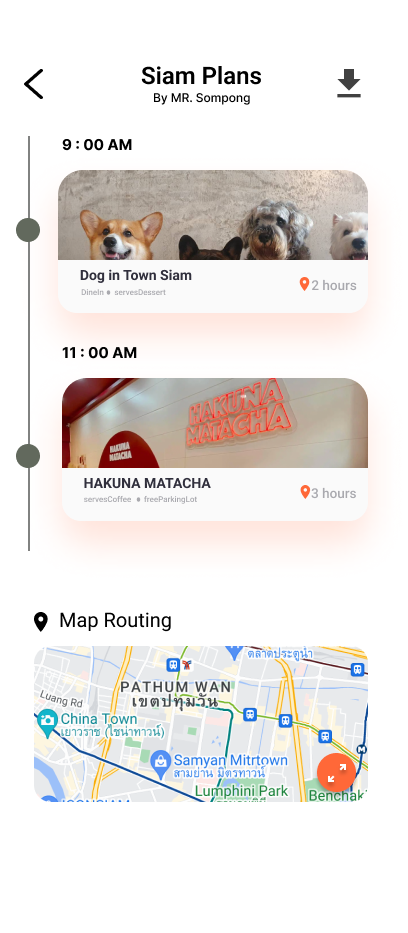
\includegraphics[width=0.5\linewidth]{chapter3/UI_Other_plan.png}
    \caption{Generated Page}
    \label{fig:Generated Page}
\end{figure}
\noindent
Figure 3-10. display the Generated Plan page of PlanADay application. After the
user selects their input and clicks on the generate plan button, the system will
suggest the plan according to the input, and all the plan details will show in this
page.

\newpage
\begin{figure}[!h]
    \centering
    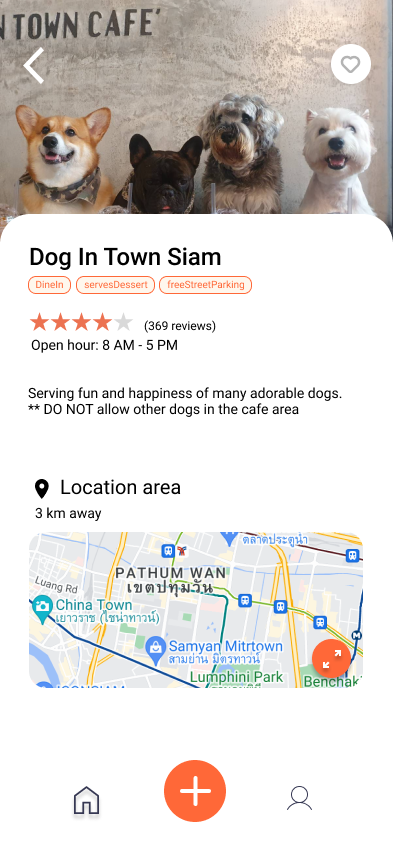
\includegraphics[width=0.5\linewidth]{chapter3/UI_Place_detail.png}
    \caption{Place Detail Page}
    \label{fig:Place Detail Page}
\end{figure}
\noindent
Figure 3-11. display the Place Detail page of PlanADay application. This page will
show after the user clicks the place card in the Generated Plan page. The details
that this page shows are place name, service types, rating, available open hours, and
location on google map.

\newpage
\begin{figure}[!h]
    \centering
    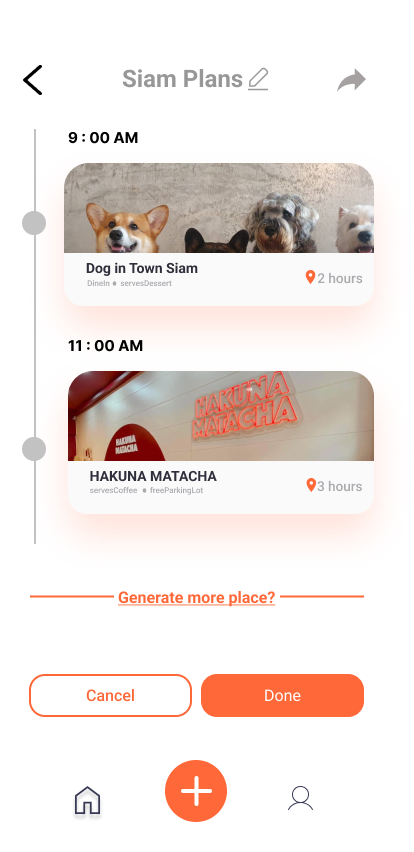
\includegraphics[width=0.5\linewidth]{chapter3/UI_Edit_plan.png}
    \caption{Edit Plan Page}
    \label{fig:Edit Plan Page}
\end{figure}
\noindent
Figure 3-12. display the Edit plan page of PlanADay application. If the user is not
satisfied with the generated plan, they can click on the edit plan button and it will
navigate to this page. Users can edit the plan name, delete each place, regenerate
the place, and add more places.

\newpage
\begin{figure}[!h]
    \centering
    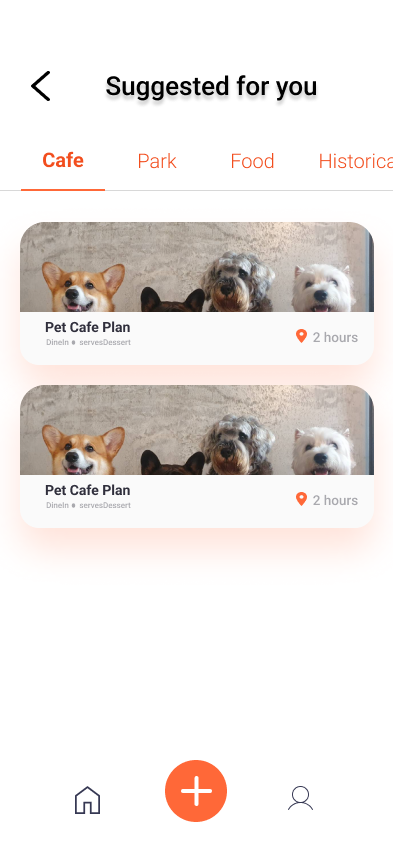
\includegraphics[width=0.5\linewidth]{chapter3/UI_Suggested_plan.png}
    \caption{Suggest Plan Page}
    \label{fig:Suggest Plan Page}
\end{figure}
\noindent
Figure 3-13. display the Suggest Plan page of PlanADay application. This page can
get on from the Homepage of the application. This page will show the plan that was
generated from others user in the application and the user can click on each plan to
see the details.

\newpage
\begin{figure}[!h]
    \centering
    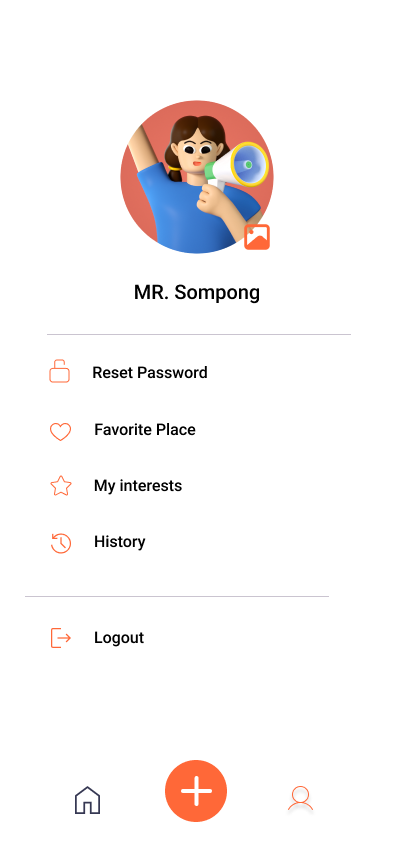
\includegraphics[width=0.5\linewidth]{chapter3/UI_User_Profile.png}
    \caption{Profile Plan Page}
    \label{fig:Profile Plan Page}
\end{figure}
\noindent
Figure 3-14. display the Profile page of PlanADay application. Users can access the
history page, persona page, and logout from their account on this profile page.

\newpage
\begin{figure}[!h]
    \centering
    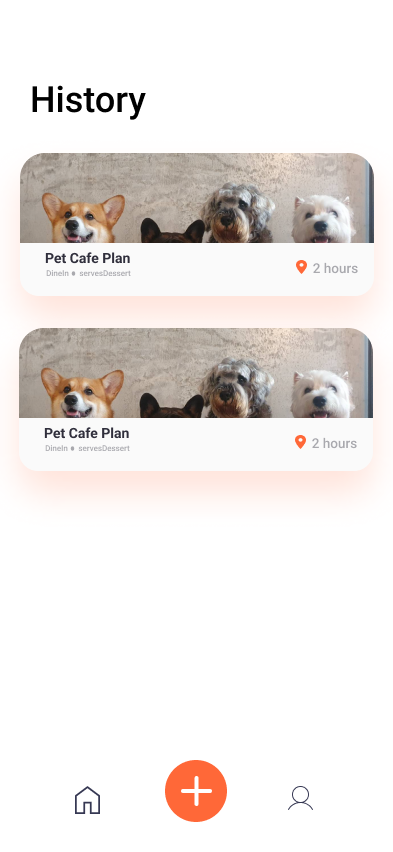
\includegraphics[width=0.5\linewidth]{chapter3/UI_History.png}
    \caption{History Page}
    \label{fig:History Page}
\end{figure}
\noindent
Figure 3-15. display the History page of PlanADay application. This page shows all
the plans that the user generated.
\newpage
\section{Database design}
\subsection{Relational Database}
\begin{figure}[!h]
	\centering
	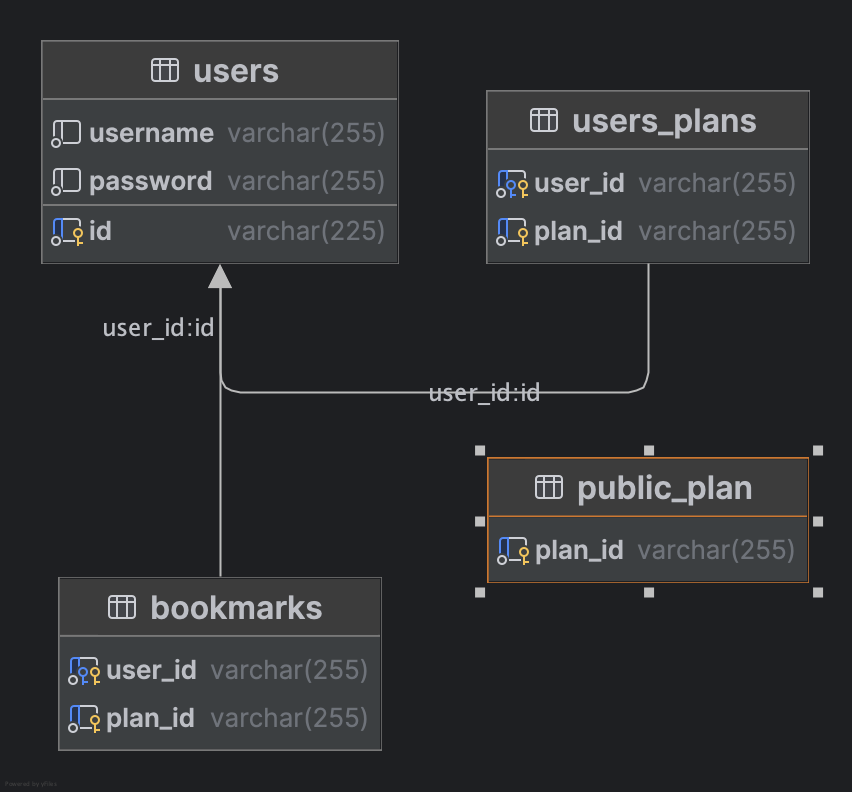
\includegraphics[width=0.5\linewidth]{chapter3/relational-database.png}
	\caption{Relational Database Schema}
	\label{fig:Relational Database Schema}
\end{figure}
Our database relies on PostgreSQL. The ER diagram illustrates a system for managing public
plans and user interactions with them. Public plans are stored in the public-plan entity, identified
by their unique plan-id. Users are represented in the users entity with their username, password,
and id. The users-plans entity establishes a many-to-many relationship between users and public
plans, allowing users to be associated with multiple plans and vice versa. The bookmarks entity
also represents a many-to-many relationship, enabling users to bookmark multiple public plans
and plans to be bookmarked by multiple users.
\newpage
\subsection{non-relational database}
\begin{figure}[!h]
    \centering
    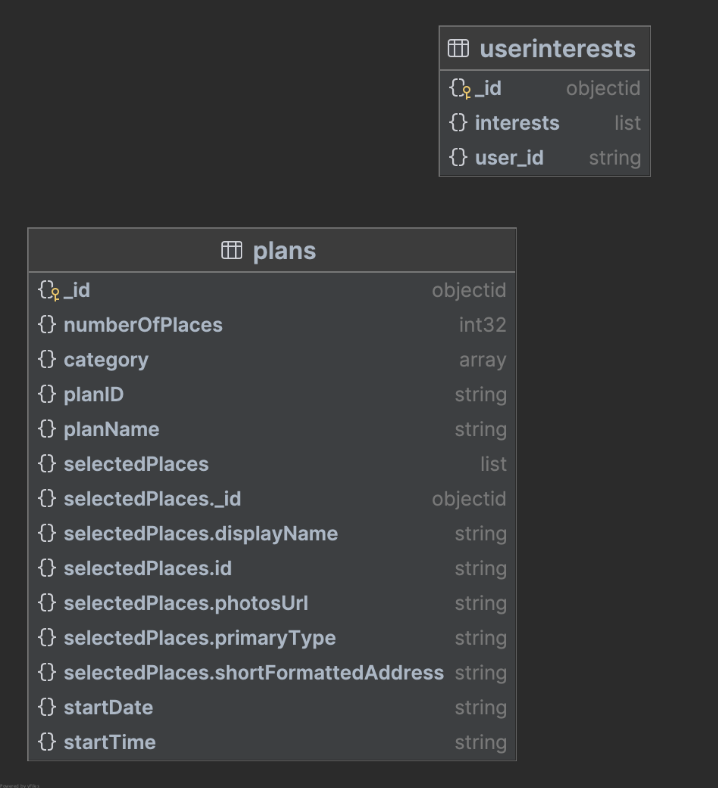
\includegraphics[width=0.6\linewidth]{chapter3/no-sql-diagram.png}
    \caption{Non-Relational Database Schema}
    \label{fig:Non-Relational Database Schema}
\end{figure}
The ER diagram depicts a database schema for managing travel plans and user interests. The
user interests table stores user IDs and their associated interests. The plans table contains detailed
information about travel plans, including the number of places, category, plan ID, name, selected
places with their attributes, and start date/time.
\chapter{System functionality}
\section{Introduction}
This chapter describes the system architecture, the plan, and the test result. First, the chapter begins with the system architecture which consists of the system functionality and main functions. The system functionality describes the components of the system and the overall structure of the system. The main function section describes all the functions in the system. Lastly, the test plan and the results explain the processes and procedures used for testing the system.
\section{4.2 System architecture}

\begin{figure}[!h]
    \centering
    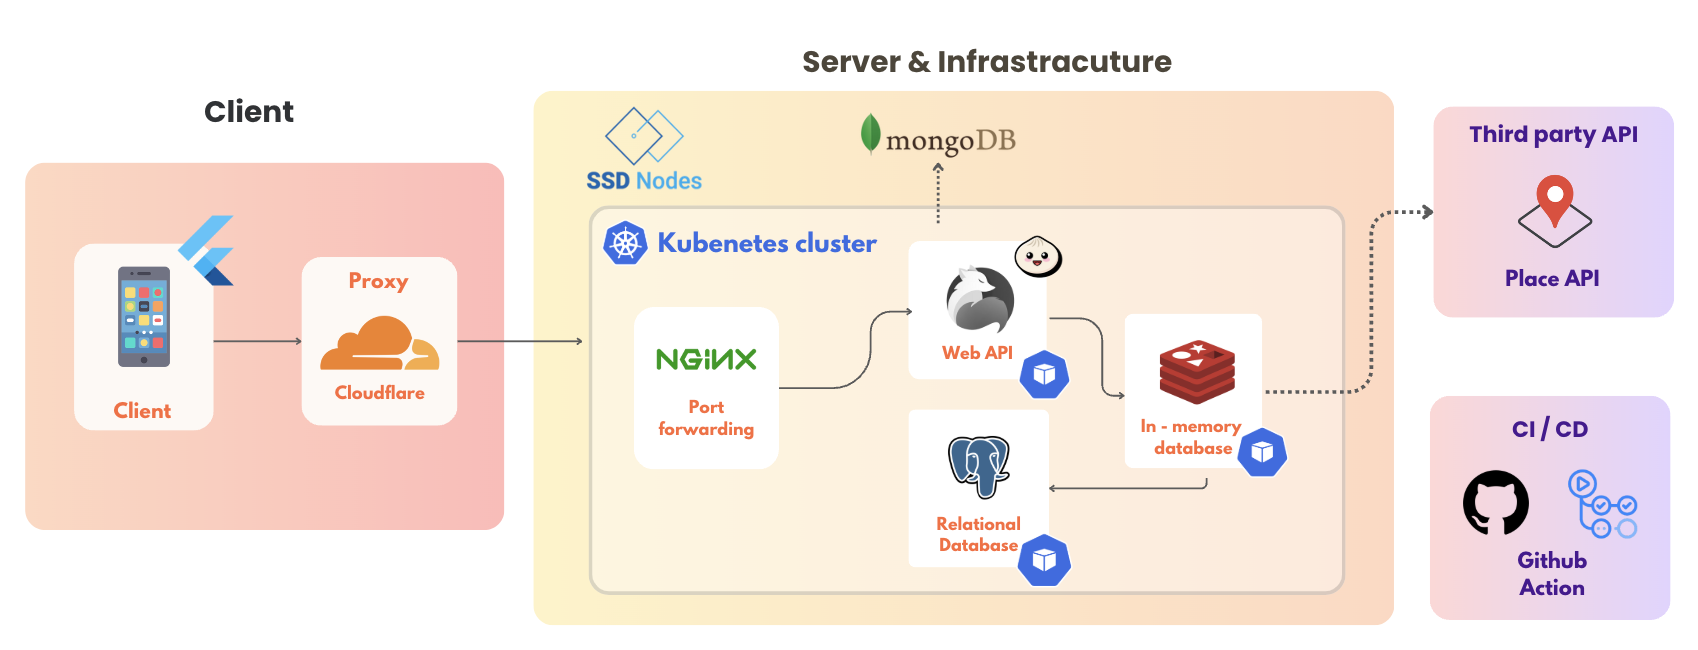
\includegraphics[width=1\linewidth]{chapter4/sysarch.png}
    \caption{System architecture}
    \label{Figure 4-1. System architecture}
\end{figure}
The PlanADay software architecture employs a client-server model, with the frontend handling user interaction through screens and forms, and the backend managing core logic, API integrations, and database operations. The frontend allows users to create plans, customize them, or authenticate via registration and login, sending input to the backend for processing. The backend retrieves data from external APIs like Google Places, caches it for efficient reuse, verifies user credentials using token-based authentication, and stores user data securely. This architecture prioritizes separation of concerns, efficiency through caching, and security, ensuring a scalable and user-friendly system for generating and customizing plans.

\newpage
\section{Test Plan}
\begin{longtable}[c]{|l|l|c|l|l|}
	\hline
	\rowcolor[HTML]{C0C0C0} 
	\multicolumn{1}{|c|}{\cellcolor[HTML]{C0C0C0}\textbf{Module}}              & \multicolumn{1}{c|}{\cellcolor[HTML]{C0C0C0}\textbf{Test Case}}                 & \textbf{Step} & \multicolumn{1}{c|}{\cellcolor[HTML]{C0C0C0}\textbf{Description}}                                                                                                                                           & \multicolumn{1}{c|}{\cellcolor[HTML]{C0C0C0}\textbf{Expected Result}}                                                                                                                                              \\ \hline
	\endfirsthead
	%
	\multicolumn{5}{c}%
	{{\bfseries Table \thetable\ continued from previous page}} \\
	\endhead
	%
	Authentication                                                             & Sign in                                                                         & 1             & \begin{tabular}[c]{@{}l@{}}Provide correct \\ credentials in the \\ sign-in form.\end{tabular}                                                                                                              & \begin{tabular}[c]{@{}l@{}}User is directed to\\ Home Screen.\end{tabular}                                                                                                                                         \\ \cline{3-5} 
																			   &                                                                                 & 2             & \begin{tabular}[c]{@{}l@{}}Provide invalid \\ credentials in the\\ sign-in form.\end{tabular}                                                                                                               & \begin{tabular}[c]{@{}l@{}}An error message, \\ "Failed to log in", is \\ displayed.\end{tabular}                                                                                                                  \\ \cline{2-5} 
																			   & Sign up                                                                         & 3             & \begin{tabular}[c]{@{}l@{}}Register a new\\ account with\\ valid credentials\end{tabular}                                                                                                                   & \begin{tabular}[c]{@{}l@{}}Registration is \\ successful, and the \\ user id directed to \\ Home screeen.\end{tabular}                                                                                             \\ \cline{3-5} 
																			   &                                                                                 & 4             & \begin{tabular}[c]{@{}l@{}}Attempt to create\\ an account with a\\ username that\\ already exists.\end{tabular}                                                                                             & \begin{tabular}[c]{@{}l@{}}An error message, "User \\ already existed", is\\ displayed.\end{tabular}                                                                                                               \\ \hline
	Home Screen                                                                & Create new plan                                                                 & 1             & \begin{tabular}[c]{@{}l@{}}Tap on the "Create\\ new plan" button\\ to initiate a new \\ trip plan.\end{tabular}                                                                                             & \begin{tabular}[c]{@{}l@{}}CreatedPlanScreen is\\ displayed.\end{tabular}                                                                                                                                          \\ \cline{2-5} 
																			   & \begin{tabular}[c]{@{}l@{}}Suggested plan\\ cards\end{tabular}                  & 2             & \begin{tabular}[c]{@{}l@{}}Tap on the suggested \\ plan card displayed\\ on the Home \\ Screen.\end{tabular}                                                                                                & \begin{tabular}[c]{@{}l@{}}Display Plan Screen with \\ plan's details.\end{tabular}                                                                                                                                \\ \cline{2-5} 
																			   & \begin{tabular}[c]{@{}l@{}}View all\\ suggested plan\end{tabular}               & 3             & \begin{tabular}[c]{@{}l@{}}Access the full list\\ of suggested plans\\ from the Home\\ Screen by tap on\\ the "View all" \\ button.\end{tabular}                                                            & \begin{tabular}[c]{@{}l@{}}Suggest Screen is \\ displayed.\end{tabular}                                                                                                                                            \\ \cline{2-5} 
																			   & Plan History                                                                    & 4             & \begin{tabular}[c]{@{}l@{}}Ensure that \\ completed plans \\ are visible on the \\ Home Screen.\end{tabular}                                                                                                & \begin{tabular}[c]{@{}l@{}}Finished plan card are\\ displayed on Home \\ Screen.\end{tabular}                                                                                                                      \\ \hline
	\begin{tabular}[c]{@{}l@{}}Generate Plan\\ Feature\end{tabular}            & \begin{tabular}[c]{@{}l@{}}Plan Generat \\ Model\end{tabular}                   & 1             & \begin{tabular}[c]{@{}l@{}}Plan Generate \\ Model that save \\ user’s plan \\ in mongoDB.\end{tabular}                                                                                                      & \begin{tabular}[c]{@{}l@{}}The plan is returned in \\ the specificed format.\end{tabular}                                                                                                                          \\ \hline
																			   & \begin{tabular}[c]{@{}l@{}}Return Places\\ from Cache\end{tabular}              & 2             & \begin{tabular}[c]{@{}l@{}}After fIll the \\ input in \\ CreatePlanScreen \\ properly and tap \\ on the “Generate” \\ button. Then \\ generate a trip \\ plan using cached \\ places.\end{tabular}          & \begin{tabular}[c]{@{}l@{}}Random places are \\ returned along with \\ a success status, if \\ data existed in the cache.\end{tabular}                                                                             \\ \cline{3-5} 
																			   &                                                                                 & 3             & \begin{tabular}[c]{@{}l@{}}Attempt to generate \\ a trip plan when the \\ requested number of \\ places exceeds the \\ cache availability.\end{tabular}                                                     & \begin{tabular}[c]{@{}l@{}}Return random places \\ and success status if data\\ is in cache. Or if there are\\ insufficient realted places\\ in the cache, appropriate\\ error handling is triggered.\end{tabular} \\ \cline{2-5} 
																			   & Nearby search                                                                   & 4             & \begin{tabular}[c]{@{}l@{}}Fetch a list of places \\ within a specified \\ distance scale \\ (e.g., 3 km) based on \\ the user's latitude\\ , longitude, and \\ selected categories.\end{tabular}           & \begin{tabular}[c]{@{}l@{}}A list of places within \\ the specified distance \\ is returned.\end{tabular}                                                                                                          \\ \cline{2-5} 
																			   & Time traveling                                                                  & 5             & \begin{tabular}[c]{@{}l@{}}Retrieve the \\ estimated travel \\ times between two \\ locations identified\\ by their “place\_id” \\ for multiple travel \\ modes (e.g., driving\\ and walking).\end{tabular} & \begin{tabular}[c]{@{}l@{}}Return an object \\ containing the travel \\ times for the specified \\ modes. And mode fails \\ are handled.\end{tabular}                                                              \\ \hline
	\begin{tabular}[c]{@{}l@{}}Customize\\ Plan Feature\end{tabular}           & \begin{tabular}[c]{@{}l@{}}Generate more\\ place\end{tabular}                   & 1             & \begin{tabular}[c]{@{}l@{}}Press on "Generate \\ More" to expand the \\ list of places in the \\ current plan.\end{tabular}                                                                                 & \begin{tabular}[c]{@{}l@{}}Additional places are \\ added to the plan based \\ on the user’s preferences \\ and location.\end{tabular}                                                                             \\ \cline{2-5} 
																			   & \begin{tabular}[c]{@{}l@{}}Regenerate\\ plan\end{tabular}                       & 2             & \begin{tabular}[c]{@{}l@{}}Tap on the \\ "Regenerate Plan" \\ button to refresh the \\ trip itinerary while \\ maintaining the \\ user’s initial input.\end{tabular}                                        & \begin{tabular}[c]{@{}l@{}}A new plan is generated,\\ replacing the previous one.\end{tabular}                                                                                                                     \\ \hline
	\begin{tabular}[c]{@{}l@{}}Suggested \\ Plan Feature\end{tabular}          & \begin{tabular}[c]{@{}l@{}}User interest \\ and plan \\ suggestion\end{tabular} & 1             & \begin{tabular}[c]{@{}l@{}}Plans from other \\ users are suggested \\ on CarouselSlider in \\ Home Screen based \\ on user interests\end{tabular}                                                           & \begin{tabular}[c]{@{}l@{}}Plans from other users \\ are suggested in the \\ CarouselSlider on the \\ Home Screen.\end{tabular}                                                                                    \\ \cline{2-5} 
																			   & \begin{tabular}[c]{@{}l@{}}Update user \\ Interests\end{tabular}                & 2             & \begin{tabular}[c]{@{}l@{}}Modify the user’s \\ preferences to update \\ plan suggestions.\end{tabular}                                                                                                     & \begin{tabular}[c]{@{}l@{}}The user’s interests are \\ updated, and relevant \\ plans are displayed on \\ the Home Screen.\end{tabular}                                                                            \\ \hline
	\begin{tabular}[c]{@{}l@{}}Publish and \\ Bookmark \\ Feature\end{tabular} & \begin{tabular}[c]{@{}l@{}}Publish the \\ plan to other \\ users.\end{tabular}  & 1             & \begin{tabular}[c]{@{}l@{}}Share a user’s plan \\ with others who have \\ similar interests.\end{tabular}                                                                                                   & \begin{tabular}[c]{@{}l@{}}The plan is published to \\ other users' suggested \\ plans.\end{tabular}                                                                                                               \\ \cline{2-5} 
																			   & \begin{tabular}[c]{@{}l@{}}Create \\ Bookmark\end{tabular}                      & 2             & \begin{tabular}[c]{@{}l@{}}Click the "Bookmark" \\ icon on a others’ plan \\ to save to the user’s \\ bookmarks.\end{tabular}                                                                               & \begin{tabular}[c]{@{}l@{}}The selected plan or \\ location is saved to \\ the user's bookmarks.\end{tabular}                                                                                                      \\ \cline{2-5} 
																			   & \begin{tabular}[c]{@{}l@{}}Delete \\ Bookmark\end{tabular}                      & 3             & \begin{tabular}[c]{@{}l@{}}Access the bookmarks \\ list and select "Delete" \\ for the desired item.\end{tabular}                                                                                           & \begin{tabular}[c]{@{}l@{}}The item is successfully \\ removed from the \\ bookmarks list.\end{tabular}                                                                                                            \\ \hline
	
	\caption{Test Plan}
	\label{tab:my-table}
\end{longtable}

	\newpage

\section{Test Results}
\begin{longtable}[c]{|l|l|l|l|c|}
	\hline
	\rowcolor[HTML]{C0C0C0} 
	\multicolumn{1}{|c|}{\cellcolor[HTML]{C0C0C0}\textbf{Module}}              & \multicolumn{1}{c|}{\cellcolor[HTML]{C0C0C0}\textbf{Test Case}}             & \multicolumn{1}{c|}{\cellcolor[HTML]{C0C0C0}\textbf{Expected Result}}                                                                                                                                              & \multicolumn{1}{c|}{\cellcolor[HTML]{C0C0C0}\textbf{Actual Result}}                                                                                       & \textbf{Status}             \\ \hline
	\endfirsthead
	%
	\multicolumn{5}{c}%
	{{\bfseries Table \thetable\ continued from previous page}} \\
	\endhead
	%
	Authentication                                                             & Sign in                                                                     & \begin{tabular}[c]{@{}l@{}}User is directed to\\ Home Screen.\end{tabular}                                                                                                                                         & \begin{tabular}[c]{@{}l@{}}Login Successfully and \\ direct to Home Screen\end{tabular}                                                                   & Passed                      \\ \cline{3-5} 
																			   &                                                                             & \begin{tabular}[c]{@{}l@{}}An error message, \\ "Failed to log in", is \\ displayed.\end{tabular}                                                                                                                  & \begin{tabular}[c]{@{}l@{}}An error message, \\ "Failed to log in," \\ is displayed.\end{tabular}                                                         & Passed                      \\ \cline{2-5} 
																			   & Sign up                                                                     & \begin{tabular}[c]{@{}l@{}}Registration is successful, \\ and the user id directed to \\ Home screeen.\end{tabular}                                                                                                & \begin{tabular}[c]{@{}l@{}}Register Successfully \\ and direct to Home \\ Screen.\end{tabular}                                                            & Passed                      \\ \cline{3-5} 
																			   &                                                                             & \begin{tabular}[c]{@{}l@{}}An error message, "User \\ already existed", is\\ displayed.\end{tabular}                                                                                                               & \begin{tabular}[c]{@{}l@{}}An error message is\\ displayed.\end{tabular}                                                                                  & Passed                      \\ \hline
	Home Screen                                                                & Create new plan                                                             & \begin{tabular}[c]{@{}l@{}}CreatedPlanScreen is\\ displayed.\end{tabular}                                                                                                                                          & \begin{tabular}[c]{@{}l@{}}The CreatePlanScreen\\ is displayed.\end{tabular}                                                                              & Passed                      \\ \cline{2-5} 
																			   & \begin{tabular}[c]{@{}l@{}}Suggested plan\\ cards\end{tabular}              & \begin{tabular}[c]{@{}l@{}}Display Plan Screen with \\ plan's details.\end{tabular}                                                                                                                                & \begin{tabular}[c]{@{}l@{}}Display Plan Screen \\ with plan’ details \\ related to the user's \\ interests.\end{tabular}                                  & Passed                      \\ \cline{2-5} 
																			   & \begin{tabular}[c]{@{}l@{}}View all\\ suggested plan\end{tabular}           & \begin{tabular}[c]{@{}l@{}}Suggest Screen is \\ displayed.\end{tabular}                                                                                                                                            & \begin{tabular}[c]{@{}l@{}}The Suggest Screen \\ is displayed.\end{tabular}                                                                               & Passed                      \\ \cline{2-5} 
																			   & Plan History                                                                & \begin{tabular}[c]{@{}l@{}}Finished plan card are\\ displayed on Home \\ -Screen.\end{tabular}                                                                                                                     & \begin{tabular}[c]{@{}l@{}}First login user has \\ no plan history {[}{]} and \\ after have created plan, \\ it displayed on Home \\ Screen.\end{tabular} & Passed                      \\ \hline
	\begin{tabular}[c]{@{}l@{}}Generate Plan\\ Feature\end{tabular}            & \begin{tabular}[c]{@{}l@{}}Plan Generat \\ Model\end{tabular}               & \begin{tabular}[c]{@{}l@{}}The plan is returned in \\ the specificed format.\end{tabular}                                                                                                                          & \begin{tabular}[c]{@{}l@{}}The received plan data \\ is returned as an object\\ in the correct format.\end{tabular}                                       & Passed                      \\ \cline{2-5} 
																			   & \begin{tabular}[c]{@{}l@{}}Return Places\\ from Cache\end{tabular}          & \begin{tabular}[c]{@{}l@{}}Random places are \\ returned along with a \\ success status, if data \\ existed in the cache.\end{tabular}                                                                             & \begin{tabular}[c]{@{}l@{}}Random places fetched \\ successfully.\end{tabular}                                                                            & Passed                      \\ \cline{3-5} 
																			   &                                                                             & \begin{tabular}[c]{@{}l@{}}Return random places \\ and success status if data\\ is in cache. Or if there are\\ insufficient realted places\\ in the cache, appropriate\\ error handling is triggered.\end{tabular} & \begin{tabular}[c]{@{}l@{}}Plan data sent \\ successfully with \\ status “success”.\end{tabular}                                                          & Passed                      \\ \hline
																			   & Nearby search                                                               & \begin{tabular}[c]{@{}l@{}}A list of places within the \\ specified distance is \\ returned.\end{tabular}                                                                                                          & \begin{tabular}[c]{@{}l@{}}A list of places within the \\ specified distance is \\ returned when the plan is \\ created.\end{tabular}                     & Passed                      \\ \cline{2-5} 
																			   & Time traveling                                                              & \begin{tabular}[c]{@{}l@{}}Return an object \\ containing the travel \\ times for the specified \\ modes. And mode fails \\ are handled.\end{tabular}                                                              & \begin{tabular}[c]{@{}l@{}}Travel time data received \\ successfully.\end{tabular}                                                                        & \multicolumn{1}{l|}{Passed} \\ \hline
	\begin{tabular}[c]{@{}l@{}}Customize \\ Plan Feature\end{tabular}          & \begin{tabular}[c]{@{}l@{}}Generate more \\ place\end{tabular}              & \begin{tabular}[c]{@{}l@{}}Additional places are \\ added to the plan \\ based on the user’s \\ preferences and \\ location.\end{tabular}                                                                          & \begin{tabular}[c]{@{}l@{}}New places are generated.\\ Failed to receive new plan \\ data is handled.\end{tabular}                                        & \multicolumn{1}{l|}{Passed} \\ \cline{2-5} 
																			   & Regenerate plan                                                             & \begin{tabular}[c]{@{}l@{}}A new plan is generated, \\ replacing the previous one.\end{tabular}                                                                                                                    & \begin{tabular}[c]{@{}l@{}}New plan is generated. \\ Failed to receive new plan \\ data is handled.\end{tabular}                                          & \multicolumn{1}{l|}{Passed} \\ \hline
	\begin{tabular}[c]{@{}l@{}}Suggested \\ Plan Feature\end{tabular}          & \begin{tabular}[c]{@{}l@{}}User interest and\\ plan suggestion\end{tabular} & \begin{tabular}[c]{@{}l@{}}Plans from other users \\ are suggested in the \\ CarouselSlider on the \\ Home Screen.\end{tabular}                                                                                    & \begin{tabular}[c]{@{}l@{}}Plans from other users \\ are displayed.\end{tabular}                                                                          & \multicolumn{1}{l|}{Passed} \\ \cline{2-5} 
																			   & \begin{tabular}[c]{@{}l@{}}Update user \\ Interests\end{tabular}            & \begin{tabular}[c]{@{}l@{}}The user’s interests are \\ updated, and relevant \\ plans are displayed on \\ the Home Screen and \\ Suggest Screen.\end{tabular}                                                      & \begin{tabular}[c]{@{}l@{}}Plans from other users \\ are displayed. On the \\ Home Screen and \\ Suggest Screen.\end{tabular}                             & \multicolumn{1}{l|}{Passed} \\ \hline
	\begin{tabular}[c]{@{}l@{}}Publish and \\ Bookmark \\ Feature\end{tabular} & \begin{tabular}[c]{@{}l@{}}Publish the plan \\ to other users.\end{tabular} & \begin{tabular}[c]{@{}l@{}}The plan is published to \\ other users' suggested \\ plans.\end{tabular}                                                                                                               & \begin{tabular}[c]{@{}l@{}}Other user's can see the \\ planthat are published.\end{tabular}                                                               & \multicolumn{1}{l|}{Passed} \\ \cline{2-5} 
																			   & Create Bookmark                                                             & \begin{tabular}[c]{@{}l@{}}The selected plan or \\ location is saved to the \\ user's bookmarks.\end{tabular}                                                                                                      & \begin{tabular}[c]{@{}l@{}}Bookmark with unique \\ plan\_id created \\ successfully.\end{tabular}                                                         & \multicolumn{1}{l|}{Passed} \\ \cline{2-5} 
																			   & Delete Bookmark                                                             & \begin{tabular}[c]{@{}l@{}}The item is successfully \\ removed from the \\ bookmarks list.\end{tabular}                                                                                                            & \begin{tabular}[c]{@{}l@{}}Bookmark with unique \\ plan\_id \\ deleted successfully\end{tabular}                                                          & \multicolumn{1}{l|}{Passed} \\ \hline
	\caption{Test Result}
	\label{tab:my-table}
\end{longtable}
\chapter{Summary and suggestions}
\section{Project Sumary}
PlanADay Application: Personalized One-Day Trip Planning System is a mobile application that
assists users in creating custom itineraries through three key types of suggestions: based on user
interests, you might be interested, and location-based recommendations. The definitions of each
suggestion are explained below.\vspace{1cm} \\
\textbf{Plan Customization:} \\
The system recommends locations that match the user’s stated preferences, such as cafes, parks,
restaurants, museums, gyms, shopping, etc. Using the user's input, including starting location,
preferred starting date and time, and desired number of stops. PlanADay generates a complete
itinerary. This feature ensures that the trip plan aligns closely with the user’s interests while
exploring nearby attractions that they have not visited before. \vspace{1cm} \\
\textbf{Completed Plans Shared by Others:} \\
This suggestion feature analyzes the user’s interests and bookmarked plans from other users to
recommend similar places they might enjoy. For instance, if a user sets their interests as cafes
and shopping, the system suggests completed plans shared by other users in the application that
align with these interests. This helps users discover new places and plans while ensuring the
recommendations remain relevant to their preferences.\par
With these features, PlanADay enables users to explore new destinations, enjoy tailored
itineraries, and make the most out of their one-day trips. It provides a seamless blend of
personalization, discovery, and flexibility.
\newpage

\section{Problems encountered and solutions}
We encountered some problems during the mobile application development phase, and some
issues took time and effort to solve. The problems encountered and solutions will discuss as
follow:
\subsection{Location fetching issue}
In our system design, we rely on the Google Maps API to fetch location data, as it provides a
comprehensive and reliable source of geolocation information worldwide. However, during
implementation, we encountered a significant challenge: the cost associated with using the
Google Cloud Platform (GCP). GCP requires users to subscribe and potentially incur charges to
access their resources, including the Google Maps API. Since cost-efficiency is a priority for us,
we explored ways to minimize expenses while maintaining functionality. After thorough
research, we discovered that Google Cloud Platform offers a \$300 free credit to new users. This
credit can be utilized without being charged unless the account is upgraded to a fully paid
subscription. By strategically registering and using this free credit, we temporarily mitigated the
cost barrier. This approach allows us to proceed with development and testing without incurring
immediate expenses. However, this solution is only temporary, and we recognize the need to plan
for long-term sustainability by either optimizing API usage or exploring alternative solutions.
Furthermore, to minimize API call costs, we are considering strategies caching frequently
accessed location data and reducing redundant API calls. These measures aim to reduce
dependency on external APIs and limit the associated expenses.

\subsection{Data storage}
The main challenge with storing location data is managing the large volume of information
fetched during the planning process. Continuously saving every fetched or edited location to the
database would consume excessive storage and increase costs unnecessarily. To address this, we
use a temporary cache to store fetched location data. Users can edit, add, or delete locations in
the cache during the planning phase. Only the finalized plan, once submitted by the user, is
stored in the database. This approach minimizes storage usage, reduces database overhead, and
ensures only relevant data is saved. The cache is also periodically cleared to free up memory.

\newpage
\begin{table}[]
    \centering
    \renewcommand{\arraystretch}{1.2} % Adjust row height for better readability
    \begin{tabular}{|p{2.2in}|p{4in}|}
    \hline
    \rowcolor[HTML]{C0C0C0} 
    \multicolumn{1}{|c|}{\cellcolor[HTML]{C0C0C0}\textbf{Suggestion}}                                                                                       & \multicolumn{1}{c|}{\cellcolor[HTML]{C0C0C0}\textbf{Details}}   \\ \hline
    Authentication & Enhance the sign-in and sign-up processes by integrating Gmail validation, moving beyond the basic username and password approach. This feature ensures a more secure and reliable authentication process for users. Additionally, incorporate third-party authentication options, such as Google, Facebook, and other social media platforms, to simplify the login process and improve user convenience and make account management more accessible and efficient. \\ \hline
    Place Pool Expansion & Efficient Filtering Algorithms: Use advanced filtering techniques to optimize the matching process and make the most of the existing pool before resorting to real-time fetching. Along with dynamic data fetching, implement a fallback mechanism to fetch additional data in real-time when the pool does not meet user requirements. This ensures that users always receive relevant suggestions. \\ \hline
    Details and more options & Enhance the detailed view of each place by providing cost estimates and more specific filters. For example, food-related locations can include details such as whether they are halal, vegan, or vegetarian-friendly. These additions offer users more clarity and enable them to customize their preferences more effectively. \\ \hline
    Recommendation Plan from others & Introduce an interactive interface for users to engage with trip plans recommended by others. Before publishing their plans, users can add comments, share experiences, and provide feedback on the plans they followed, fostering collaboration and building a more engaging community within the application. \\ \hline
    Frontend \& Backend Code quality & Apply other higher-efficiency techniques to build the large-scale recommendation system both frontend and backend. \\ \hline
    \end{tabular}
    \caption{List of Suggestions for further development}
    \label{tab:suggestion-table}
\end{table}




% \cite{google_maps}
% \cite{huang2018}
% \cite{wins2024}

\bibliographystyle{plain}
\bibliography{references/references}
\addcontentsline{toc}{chapter}{REFERRENCES}

\end{document}
